% Options for packages loaded elsewhere
% Options for packages loaded elsewhere
\PassOptionsToPackage{unicode}{hyperref}
\PassOptionsToPackage{hyphens}{url}
\PassOptionsToPackage{dvipsnames,svgnames,x11names}{xcolor}
%
\documentclass[
  letterpaper,
  DIV=11,
  numbers=noendperiod]{scrreprt}
\usepackage{xcolor}
\usepackage{amsmath,amssymb}
\setcounter{secnumdepth}{5}
\usepackage{iftex}
\ifPDFTeX
  \usepackage[T1]{fontenc}
  \usepackage[utf8]{inputenc}
  \usepackage{textcomp} % provide euro and other symbols
\else % if luatex or xetex
  \usepackage{unicode-math} % this also loads fontspec
  \defaultfontfeatures{Scale=MatchLowercase}
  \defaultfontfeatures[\rmfamily]{Ligatures=TeX,Scale=1}
\fi
\usepackage{lmodern}
\ifPDFTeX\else
  % xetex/luatex font selection
\fi
% Use upquote if available, for straight quotes in verbatim environments
\IfFileExists{upquote.sty}{\usepackage{upquote}}{}
\IfFileExists{microtype.sty}{% use microtype if available
  \usepackage[]{microtype}
  \UseMicrotypeSet[protrusion]{basicmath} % disable protrusion for tt fonts
}{}
\makeatletter
\@ifundefined{KOMAClassName}{% if non-KOMA class
  \IfFileExists{parskip.sty}{%
    \usepackage{parskip}
  }{% else
    \setlength{\parindent}{0pt}
    \setlength{\parskip}{6pt plus 2pt minus 1pt}}
}{% if KOMA class
  \KOMAoptions{parskip=half}}
\makeatother
% Make \paragraph and \subparagraph free-standing
\makeatletter
\ifx\paragraph\undefined\else
  \let\oldparagraph\paragraph
  \renewcommand{\paragraph}{
    \@ifstar
      \xxxParagraphStar
      \xxxParagraphNoStar
  }
  \newcommand{\xxxParagraphStar}[1]{\oldparagraph*{#1}\mbox{}}
  \newcommand{\xxxParagraphNoStar}[1]{\oldparagraph{#1}\mbox{}}
\fi
\ifx\subparagraph\undefined\else
  \let\oldsubparagraph\subparagraph
  \renewcommand{\subparagraph}{
    \@ifstar
      \xxxSubParagraphStar
      \xxxSubParagraphNoStar
  }
  \newcommand{\xxxSubParagraphStar}[1]{\oldsubparagraph*{#1}\mbox{}}
  \newcommand{\xxxSubParagraphNoStar}[1]{\oldsubparagraph{#1}\mbox{}}
\fi
\makeatother


\usepackage{longtable,booktabs,array}
\usepackage{calc} % for calculating minipage widths
% Correct order of tables after \paragraph or \subparagraph
\usepackage{etoolbox}
\makeatletter
\patchcmd\longtable{\par}{\if@noskipsec\mbox{}\fi\par}{}{}
\makeatother
% Allow footnotes in longtable head/foot
\IfFileExists{footnotehyper.sty}{\usepackage{footnotehyper}}{\usepackage{footnote}}
\makesavenoteenv{longtable}
\usepackage{graphicx}
\makeatletter
\newsavebox\pandoc@box
\newcommand*\pandocbounded[1]{% scales image to fit in text height/width
  \sbox\pandoc@box{#1}%
  \Gscale@div\@tempa{\textheight}{\dimexpr\ht\pandoc@box+\dp\pandoc@box\relax}%
  \Gscale@div\@tempb{\linewidth}{\wd\pandoc@box}%
  \ifdim\@tempb\p@<\@tempa\p@\let\@tempa\@tempb\fi% select the smaller of both
  \ifdim\@tempa\p@<\p@\scalebox{\@tempa}{\usebox\pandoc@box}%
  \else\usebox{\pandoc@box}%
  \fi%
}
% Set default figure placement to htbp
\def\fps@figure{htbp}
\makeatother





\setlength{\emergencystretch}{3em} % prevent overfull lines

\providecommand{\tightlist}{%
  \setlength{\itemsep}{0pt}\setlength{\parskip}{0pt}}



 


\KOMAoption{captions}{tableheading}
\makeatletter
\@ifpackageloaded{bookmark}{}{\usepackage{bookmark}}
\makeatother
\makeatletter
\@ifpackageloaded{caption}{}{\usepackage{caption}}
\AtBeginDocument{%
\ifdefined\contentsname
  \renewcommand*\contentsname{Table of contents}
\else
  \newcommand\contentsname{Table of contents}
\fi
\ifdefined\listfigurename
  \renewcommand*\listfigurename{List of Figures}
\else
  \newcommand\listfigurename{List of Figures}
\fi
\ifdefined\listtablename
  \renewcommand*\listtablename{List of Tables}
\else
  \newcommand\listtablename{List of Tables}
\fi
\ifdefined\figurename
  \renewcommand*\figurename{Figure}
\else
  \newcommand\figurename{Figure}
\fi
\ifdefined\tablename
  \renewcommand*\tablename{Table}
\else
  \newcommand\tablename{Table}
\fi
}
\@ifpackageloaded{float}{}{\usepackage{float}}
\floatstyle{ruled}
\@ifundefined{c@chapter}{\newfloat{codelisting}{h}{lop}}{\newfloat{codelisting}{h}{lop}[chapter]}
\floatname{codelisting}{Listing}
\newcommand*\listoflistings{\listof{codelisting}{List of Listings}}
\makeatother
\makeatletter
\makeatother
\makeatletter
\@ifpackageloaded{caption}{}{\usepackage{caption}}
\@ifpackageloaded{subcaption}{}{\usepackage{subcaption}}
\makeatother
\usepackage{bookmark}
\IfFileExists{xurl.sty}{\usepackage{xurl}}{} % add URL line breaks if available
\urlstyle{same}
\hypersetup{
  pdftitle={African Center Annual Report 2023 - 2024},
  colorlinks=true,
  linkcolor={blue},
  filecolor={Maroon},
  citecolor={Blue},
  urlcolor={Blue},
  pdfcreator={LaTeX via pandoc}}


\title{African Center Annual Report 2023 - 2024}
\usepackage{etoolbox}
\makeatletter
\providecommand{\subtitle}[1]{% add subtitle to \maketitle
  \apptocmd{\@title}{\par {\large #1 \par}}{}{}
}
\makeatother
\subtitle{African Center For Governance Asset Recovery And Sustainable
Development}
\author{}
\date{}
\begin{document}
\maketitle

\renewcommand*\contentsname{Table of contents}
{
\hypersetup{linkcolor=}
\setcounter{tocdepth}{4}
\tableofcontents
}

\bookmarksetup{startatroot}

\chapter*{About}\label{about}
\addcontentsline{toc}{chapter}{About}

\markboth{About}{About}

\phantomsection\label{hero-heading}

The African Center for Governance, Asset Recovery, and Sustainable
Development (the African Center) is an independent civil society
organization headquartered in Abuja, Nigeria. The Center works with
national governments, international and regional organizations, and
non-governmental organizations to promote good governance, sustainable
development, and the rule of law. We work to foster national and
international cooperation in the recovery and return of proceeds of
corruption and illicit financial flow to fill funding gaps for
implementing the SDGs. The African Center shares the view that returning
stolen assets will enable countries in the global South, particularly
Africa, to build a foundation for prosperity, and good governance.

The African Center fosters national and international cooperation in the
recovery and return of the proceeds of criminal activity to enable
countries to address inequality, reduce poverty, innovate, and build
sustainable partnerships. We aim to promote good governance, sustainable
development, and the rule of law. This is achieved through training,
research, program management, strategy development, international
cooperation, and promoting anti-corruption and anti-money laundering
regulatory compliance.

\subsection*{Capacity Statement}\label{capacity-statement}
\addcontentsline{toc}{subsection}{Capacity Statement}

Since 2022, the African Center has advanced governance, asset recovery
transparency, and justice sector accountability. Partnering with global
and regional organizations, we have trained legal and financial
professionals across Africa in asset tracing and financial crime
management.

Our work focuses on anti-corruption, anti-money laundering,
counter-financing of terrorism and countering proliferation
financing(AML/CFT/CPF). Collaborating with the Nigerian Bar Association
(NBA) and Nigerian Financial Intelligence Unit, we enhance compliance
through research, risk assessment, and policy guidance. Our Executive
Director serves on key NBA committees to strengthen legal sector
compliance.

We support Nigerian agencies in addressing FATF grey list deficiencies
through training and international cooperation efforts with the Global
South Dialogue on Economic Crime (GSDEC). To sustain research and
training, we have agreements with institutions like Nigerian Institute
of Advanced Legal Studies (NIALS), Digital Evidence Forensics and
Compliance Institute (DEFCI), and the Nigerian Bar Association (NBA).

Our research covers illicit financial flows, justice reforms, and asset
recovery, aligning with Agenda 2063. We have published a compendium on
anti-corruption best practices and are working with Nigeria's Ministry
of Justice on UN anti-corruption initiatives. Our Open Asset Database
maps African asset recovery data.

We partner with UNODC, the World Bank, and the UNCAC Coalition to shape
an African-centric asset recovery approach. In collaboration with IBLF
Global, we are developing a CSO Advocacy Toolkit under Transparency
International's REAP project and advising the African Development Bank
on asset management.

\paragraph*{\texorpdfstring{\textbf{Mission}}{Mission}}\label{mission}
\addcontentsline{toc}{paragraph}{\textbf{Mission}}

Our mission is to reinforce the links between governance, asset
recovery, and sustainable development goals in line with Agenda 2030 and
the promotion of the rule of law, strengthening justice institutions,
preventing illicit financial flows, recovering stolen assets, and social
reuse of stolen assets.

\paragraph*{\texorpdfstring{\textbf{Vision}}{Vision}}\label{vision}
\addcontentsline{toc}{paragraph}{\textbf{Vision}}

We envision a world free from illicit financial flows, where proceeds of
crime are recovered and returned to the victims of corruption to improve
livelihood and reduce poverty and inequality.~

\section*{Thematic Objectives}\label{thematic-objectives}
\addcontentsline{toc}{section}{Thematic Objectives}

\markright{Thematic Objectives}

\begin{center}
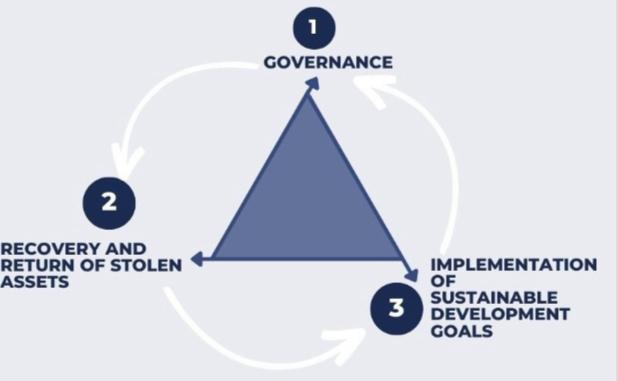
\includegraphics[width=5.20833in,height=\textheight,keepaspectratio]{images/about/thematic_objectives.jpg}
\end{center}

\subsection*{Strengthening Governance and Accountability for Sustainable
Development}\label{strengthening-governance-and-accountability-for-sustainable-development}
\addcontentsline{toc}{subsection}{Strengthening Governance and
Accountability for Sustainable Development}

At the African Center, we are committed to advancing good governance and
accountability across Africa by aligning our efforts with the United
Nations Sustainable Development Goals (SDGs). Our approach goes beyond
policy advocacy. We drive real change by ensuring citizens, especially
women, have access to quality education, justice, and economic
empowerment tools.

This year, we focused on breaking systemic barriers that hinder
inclusive development. Through targeted initiatives, we challenged
harmful social norms, expanded economic opportunities, and leveraged
technology to address the unique needs of women. By working at the
intersection of governance, gender equity, and innovation, we are
building stronger,

\subsection*{Recovery and Return of Stolen
Assets}\label{recovery-and-return-of-stolen-assets}
\addcontentsline{toc}{subsection}{Recovery and Return of Stolen Assets}

Under the Asset Recovery theme, the African Center works with national,
regional, and international organizations and professional bodies in the
private and public sectors to develop clear and comprehensive legal
frameworks for recovering the proceeds of all forms of crime and
transparently managing the returned assets for the benefit of the
victims of these crimes. Our efforts align with Chapter V of the
\href{https://www.unodc.org/documents/brussels/UN_Convention_Against_Corruption.pdf}{United
Nations Convention against Corruption (UNCAC)}, the
\href{https://au.int/sites/default/files/treaties/36382-treaty-0028_-_african_union_convention_on_preventing_and_combating_corruption_e.pdf}{African
Union Convention on Preventing and Combatting Corruption (AUCPCC)}, and
the
\href{https://au.int/sites/default/files/newsevents/workingdocuments/43786-wd-42297-doc-COMMON-AFRICAN-POSITION-ON-ASSEST-RECOVERY-ENGLISH-NEWLY-PROOFREAD-1.pdf}{Common
African Position on Asset Recovery (CAPAR).} The Center's core
objectives are to identify the links between the return of proceeds of
crime and sustainable development and to work with countries of the
global South to advocate for expedited mechanisms to return stolen
assets for the benefit of their citizens.

\subsection*{Implementation of the United Nations Sustainable
Development
Goals}\label{implementation-of-the-united-nations-sustainable-development-goals}
\addcontentsline{toc}{subsection}{Implementation of the United Nations
Sustainable Development Goals}

At the African Center for Governance and Asset Recovery, we are at the
forefront of strengthening asset recovery systems to ensure that stolen
wealth is returned and used for the benefit of socio-economic growth.
The Center works with development partners and other civil society
organizations to ensure the effective implementation of the
\href{https://sdgs.un.org/goals}{United Nations Sustainable Development
Goals} (UN/SDGs) and the African Union
(\href{https://au.int/en/agenda2063/overview}{AU) Agenda 2063}. We focus
specifically on UN SDG Goal 16 and AU Agenda Goals 11 and 12. Our aim is
to ``promote peaceful and inclusive societies for sustainable
development, provide access to justice for all, and build effective,
accountable, and inclusive institutions at all levels''. The African
Center's work in this thematic area is closely linked to the governance
and asset recovery thematic areas.

\section*{Organogram}\label{organogram}
\addcontentsline{toc}{section}{Organogram}

\markright{Organogram}

\begin{center}
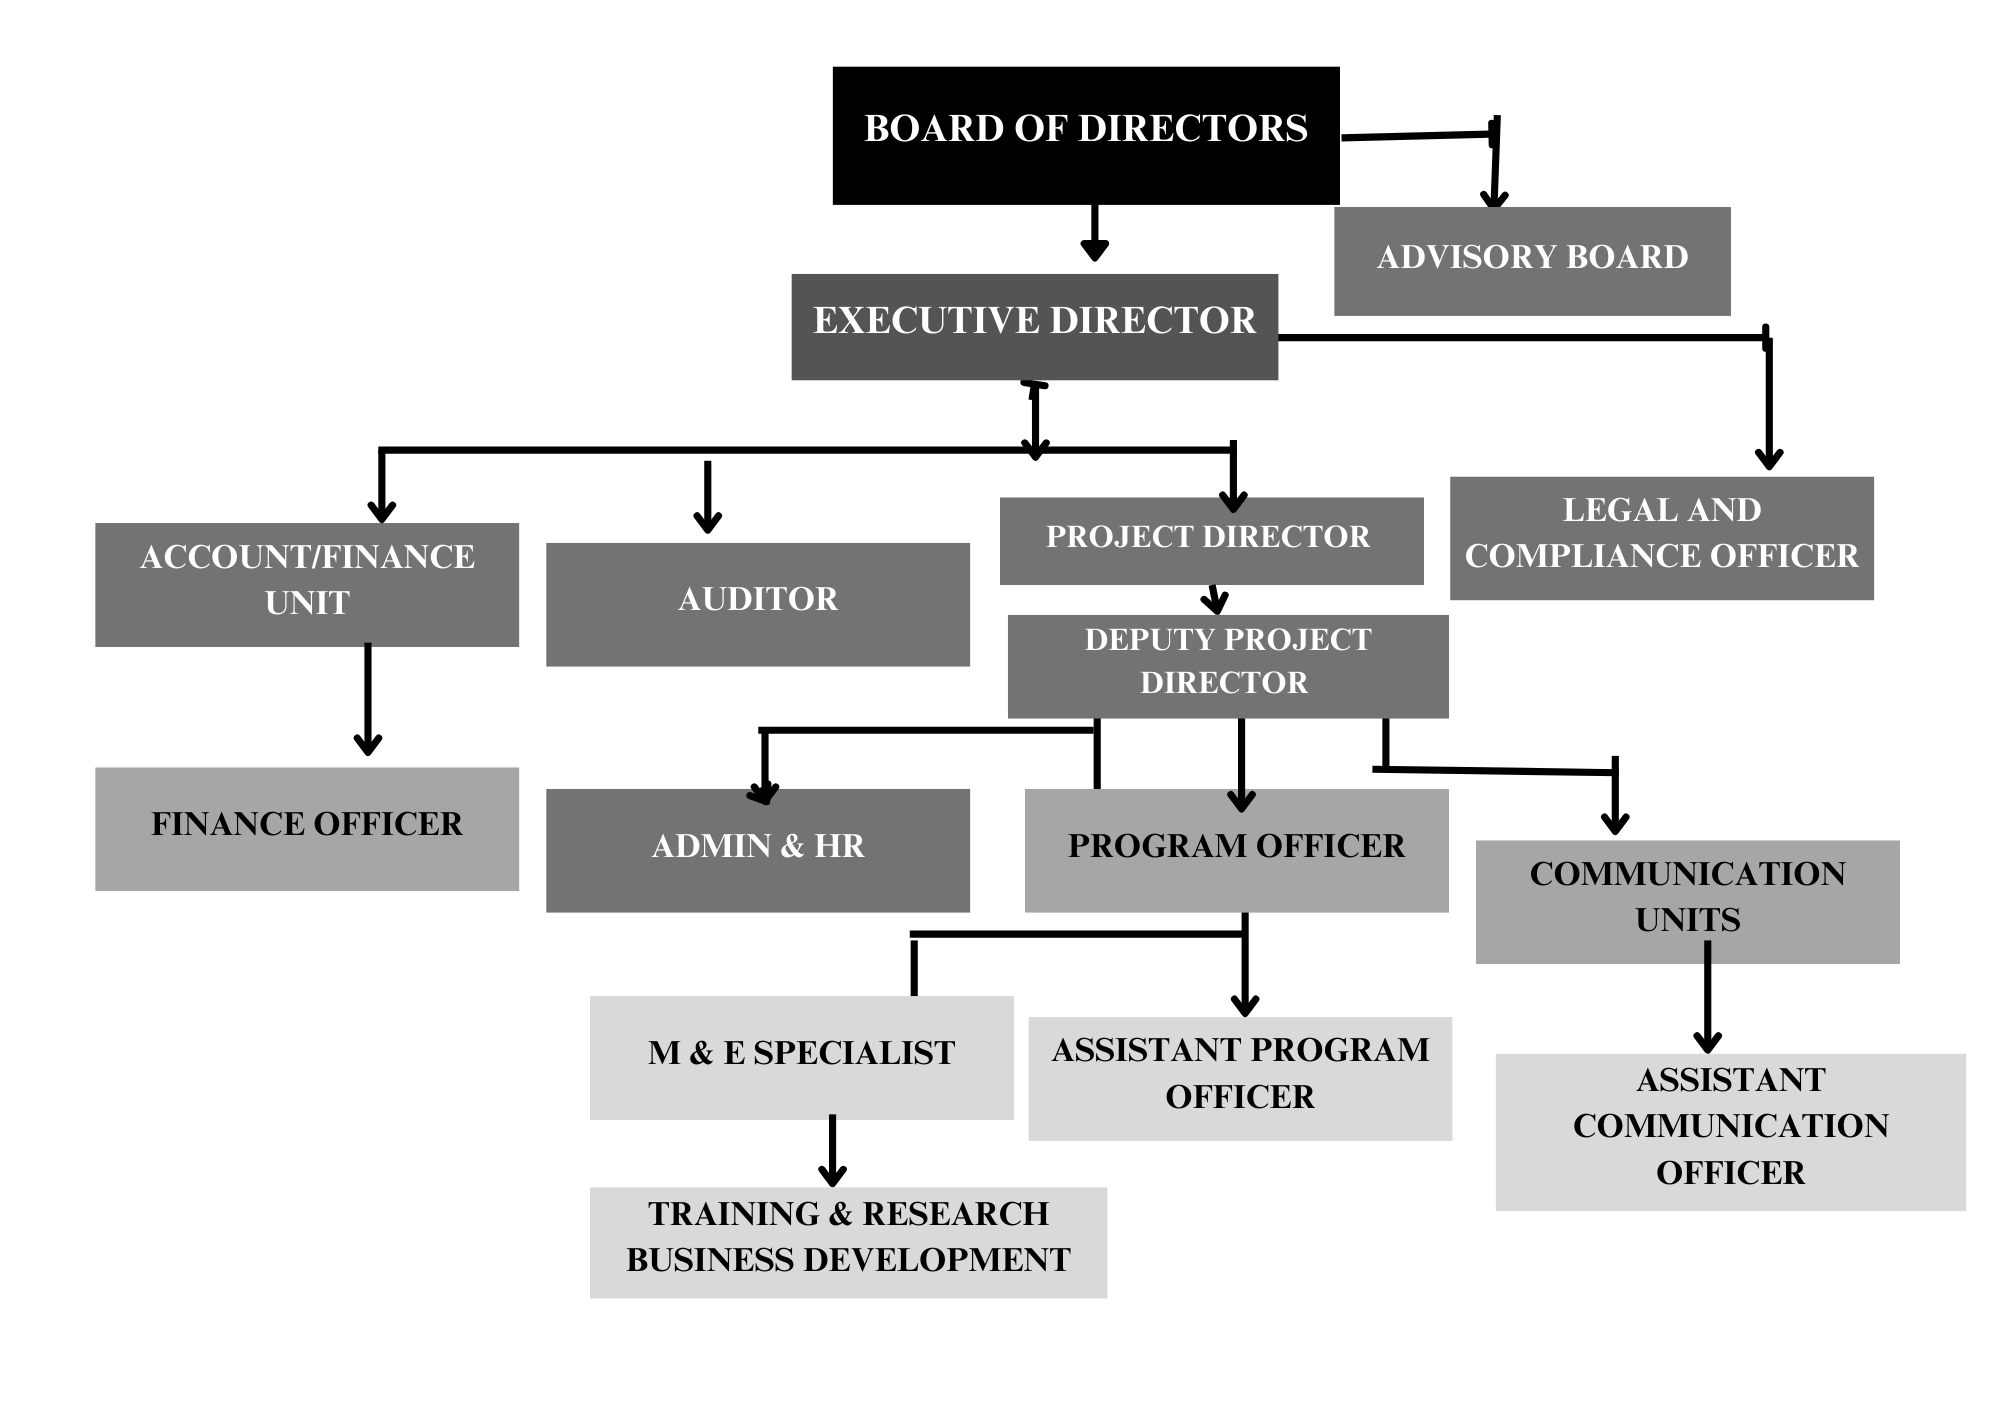
\includegraphics[width=5.20833in,height=\textheight,keepaspectratio]{images/about/organogram.png}
\end{center}

\part{Preface}

\chapter*{Statement from the Chairman of the Board of
Directors}\label{statement-from-the-chairman-of-the-board-of-directors}
\addcontentsline{toc}{chapter}{Statement from the Chairman of the Board
of Directors}

\markboth{Statement from the Chairman of the Board of
Directors}{Statement from the Chairman of the Board of Directors}

Dear Stakeholders,

As we reflect on the past year, I am both proud and inspired by the
resilience and dedication of our organization in promoting good
governance and sustainable development in the legal sector. Our mission
to promote transparency, accountability, and the rule of law has never
been more critical, and I am honoured to present this annual report,
which highlights our achievements, challenges, and the path forward.

However, the challenges we face are significant. The global landscape of
democratic governance is evolving, and we must remain vigilant and
adaptable. In response, we have fortified our commitment to advocacy and
legal support for those who stand against corruption.

Looking ahead, we are excited to embark on new initiatives that will
further our impact. We will continue to invest in research and
data-driven advocacy, ensuring that our strategies are informed by
evidence and best practices. Additionally, we are committed to enhancing
our capacity-building programs, as well as equipping individuals and
organizations with the tools they need to combat corruption effectively.

I would like to extend my heartfelt gratitude to our partners, dedicated
staff, board members, volunteers, and supporters. Your unwavering
commitment and passion for our goals are the driving forces behind our
success. Additionally, we would like to welcome our new advisory board
members. Together, we are making a difference and will continue to
strive for a world where integrity prevails.

As we move forward, let us remain united in our mission. Fighting
impunity, money laundering, and financial and organized crimes is not
just a challenge; it is an opportunity to build a more just and
equitable society for all. Thank you for your continued support and
belief in our vision.

Sincerely,\\

\textbf{Jideani Agabaidu}\\
\emph{Chairman of the Board}\\
\emph{African Center for Governance, Asset Recovery and Sustainable
Development}\\

\chapter*{Statement from the Executive
Director}\label{statement-from-the-executive-director}
\addcontentsline{toc}{chapter}{Statement from the Executive Director}

\markboth{Statement from the Executive Director}{Statement from the
Executive Director}

\subsection*{\texorpdfstring{\emph{Setting The Course For 2025 - A Year
In
Review}}{Setting The Course For 2025 - A Year In Review}}\label{setting-the-course-for-2025---a-year-in-review}
\addcontentsline{toc}{subsection}{\emph{Setting The Course For 2025 - A
Year In Review}}

As 2024 ends, we reflect on a year of significant achievements and
persistent challenges in our fight against illicit financial flows
(IFFs) and their impact on governance and sustainable development across
Africa. At the African Center, we remain steadfast in our commitment to
promoting transparency, accountability, and good governance, guided by
the principles of the United Nations Sustainable Development Goals (UN
SDGs), particularly Goal 16, on Peace, Justice and Strong Institutions.
We are also guided by the African Union 2063 Agenda, the Common Africa
Position on Asset Recovery and the Global Framework on Asset Recovery.

This past year has underscored the urgent need for our work. It is well
documented that corruption, IFFs, and money laundering erode public
trust, divert crucial resources from development priorities, and
exacerbate inequalities. The intricate web of illicit financial flows,
often facilitated by complex transnational networks, deprives nations of
vital funds needed to invest in education, healthcare, and
infrastructure, hindering progress toward the SDGs.

This report details our key activities and accomplishments over the past
year in response to this threat. In this annual report - our first - you
will read about our impactful research, advocacy efforts,
capacity-building programs, and strategic partnerships. We are proud of
our progress in contributing to the efforts to remove Nigeria from the
Financial Action Task Force (FATF) greylist through collaboration with
the Nigeria Legal Professionals. This collaboration led to the drafting
of the anti-money laundering risk assessment for the legal sector in
Nigeria, the development of an anti-money laundering reporting portal,
the drafting of guidance on the role of civil society in asset recovery,
the drafting of an asset recovery policy manual for the Federal Ministry
of Justice.

Finally, this collaboration enabled us to supportAfrican institutions
and non-state actors to address weak governance structures. These
successes are a testament to the dedication and expertise of our team,
the unwavering support of our partners, and the resilience of the
communities we serve.

Significant obstacles remain, including the complexity of cross-border
investigations, limited political will, and lack of resources. To
overcome these challenges, we must continue to innovate, collaborate,
and strengthen our collective efforts. Looking ahead, we are committed
to deepening our impact by leveraging technology through our open assets
database, expanding our reach to new regions, and strengthening
collaboration with government agencies. We will continue to champion the
principles of transparency and accountability, working tirelessly to
ensure that proceeds of criminal activities are recovered and returned
to their rightful owners. We invite you to explore this report and learn
more about our work. We are deeply grateful to our partners,
particularly the MacArthur Foundation, the Foreign and the Commonwealth
Development Office (UK FCDO) and German GIZ. Your support is essential
to the sustenance of our mission. Our progress over the past months
would not have been possible without the dedication of our board and
staff. I am genuinely grateful for your time and expertise in advancing
the African Center's mission.

Together, we can build a future where the principles of justice, the
rule of law, good governance and sustainable development prevail.I look
forward to continuing our collective efforts in the years ahead.

Sincerely,\\
\textbf{Juliet Ibekaku-Nwagwu}\\
\emph{Founder \& Executive Director}\\
\emph{African Center for Governance Asset Recovery and Sustainable
Development}

\part{Highlights from the Year 2024: Core Areas of Engagement}

\chapter{Strengthening Governance and Accountability for Sustainable
Development}\label{strengthening-governance-and-accountability-for-sustainable-development-1}

In 2023 and 2024, the African Center advanced its mission through
capacity building, stakeholder engagement, and policy advocacy. Key
initiatives included training investigative journalists on asset
recovery and FATF methodologies, collaborating with global institutions
to combat financial crime, and launching guidelines for civil society
organizations on managing proceeds of crime. Through high-level
engagements, risk assessment workshops, and international partnerships,
the Center reinforced its commitment to transparency, accountability,
and strengthening Nigeria's financial integrity.

\subsection{Speaker: Nigerian Bar Association, Bwari
Branch}\label{speaker-nigerian-bar-association-bwari-branch}

The African Center for Governance, Asset Recovery, and Sustainable
Development joined the Law Reform Committee of the Nigerian Bar
Association (NBA) Bwari Branch as a panelist in the one-day symposium on
Anti-Corruption on December 8, 2023.

The symposium, themed ``Anti-Corruption Fight in Nigeria: A Lost Battle
or a Work in Progress?'' aligns with the global efforts to address the
issue of pervasive corruption and to mark International Anti-Corruption
Day on December 9, 2023.\\
It provided a platform for stakeholders to deliberate on the state of
Nigeria's anti-corruption initiatives and chart a course for future
progress. Perspectives and insights on the challenges and successes
encountered in Nigeria's ongoing battle against corruption was shared.

\begin{center}
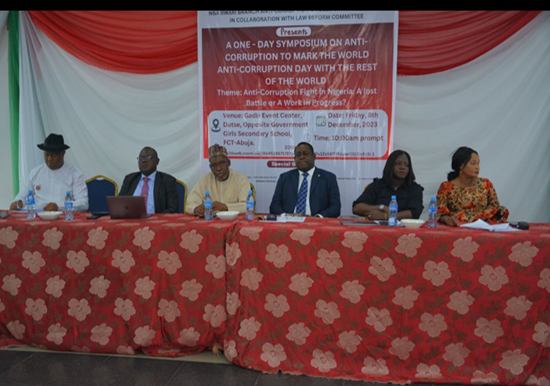
\includegraphics[width=4.16667in,height=\textheight,keepaspectratio]{images/strengthen/00_strength_gov.png}
\end{center}

\subsection{Training: Counter Financing of Terrorism Specialists at the
International Institute for Justice and Rule of
Law}\label{training-counter-financing-of-terrorism-specialists-at-the-international-institute-for-justice-and-rule-of-law}

On 21-23rd November 2023, the African Center facilitated three sessions
at the National Training on Countering the Financing of Terrorism
organized by The International Institute for Justice and Rule of Law
(IIJ) in Abuja, Nigeria.\\
\strut ~\\
The three-day national-level training program was aimed at building the
capacities of investigators, prosecutors, judges, financial analysts,
and regulatory authorities and promoting inter-agency cooperation and
public-private dialogue. It sought to equip key CFT actors in Nigeria
with comprehensive knowledge and practical strategies to counter the
financing of terrorism within the country effectively. Additionally, the
training was aimed to align the national CFT framework with FATF
requirements with expected outcomes, including an enhanced understanding
of Nigeria's specific terrorist financing vulnerabilities and tools to
address them; improved knowledge of tools and techniques for
identifying, tracking, and disrupting terrorist financing networks, in
particular involving high-risk sectors; and improved interagency
cooperation and public-private dialogue on CFT. Vulnerabilities within
the nation's high-risk sector of Designated Non-Financial Businesses and
Professions (DNFBPs), Non-Profits, and Virtual Assets were also
addressed.

\begin{figure}

\begin{minipage}{0.47\linewidth}
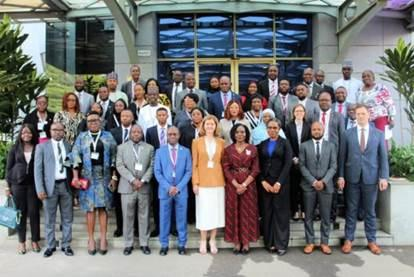
\includegraphics[width=3.64583in,height=\textheight,keepaspectratio]{images/strengthen/01_bwari.jpg}\end{minipage}%
%
\begin{minipage}{0.53\linewidth}
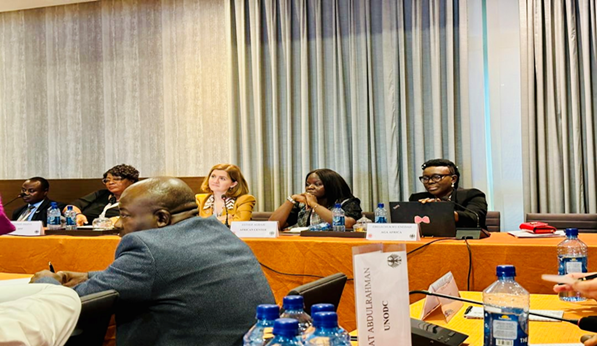
\includegraphics[width=4.16667in,height=\textheight,keepaspectratio]{images/strengthen/01_2_bwari.png}\end{minipage}%

\end{figure}%

~~

\subsection{Facilitation: Webinar with the Compliance Institute of
Nigeria}\label{facilitation-webinar-with-the-compliance-institute-of-nigeria}

On 5 July 2023, the Compliance Institute of Nigeria (CIN) in
collaboration with the African Center for Governance, held a webinar
titled ``Recent Anti-Money Laundering/Countering the Financing of
Terrorism (AML/CFT) Regulatory and Legal Frameworks in Nigeria: How to
Use a Risk-Based Approach to Onboard Customer''.

Three hundred and forty participants attended the webinar including law
enforcement agencies, bankers, compliance officers, and compliance
enthusiasts. Key issues on the recent AML/CFT legal frameworks and
risk-based approach were discussed by speakers from the Special Control
Unit on Money Laundering (SCUML), the Nigerian Financial Intelligence
Unit (NFIU), and the African Center.

\begin{center}
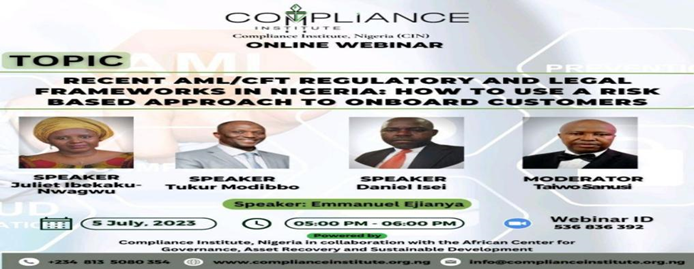
\includegraphics[width=3.125in,height=2.08333in]{images/strengthen/02_counterfinance.png}
\end{center}

\subsection{Facilitation: Session with the Global South Dialogue on
Economic
Crime}\label{facilitation-session-with-the-global-south-dialogue-on-economic-crime}

In February 2024, the African Center facilitated a session at the GSDEC
workshop, ``A Multistakeholder Approach to Nigeria's FATF Delisting''.
The event brought together stakeholders to discuss challenges and
strategies for Nigeria's removal from the grey list.

The session highlighted the critical role of leadership in promoting
good governance and combating financial crimes. Drawing from past
experience in corruption investigations and Nigeria's 2013 delisting,
the discussion reinforced the African Center's commitment to
transparency, accountability, and economic crime prevention.

\begin{center}
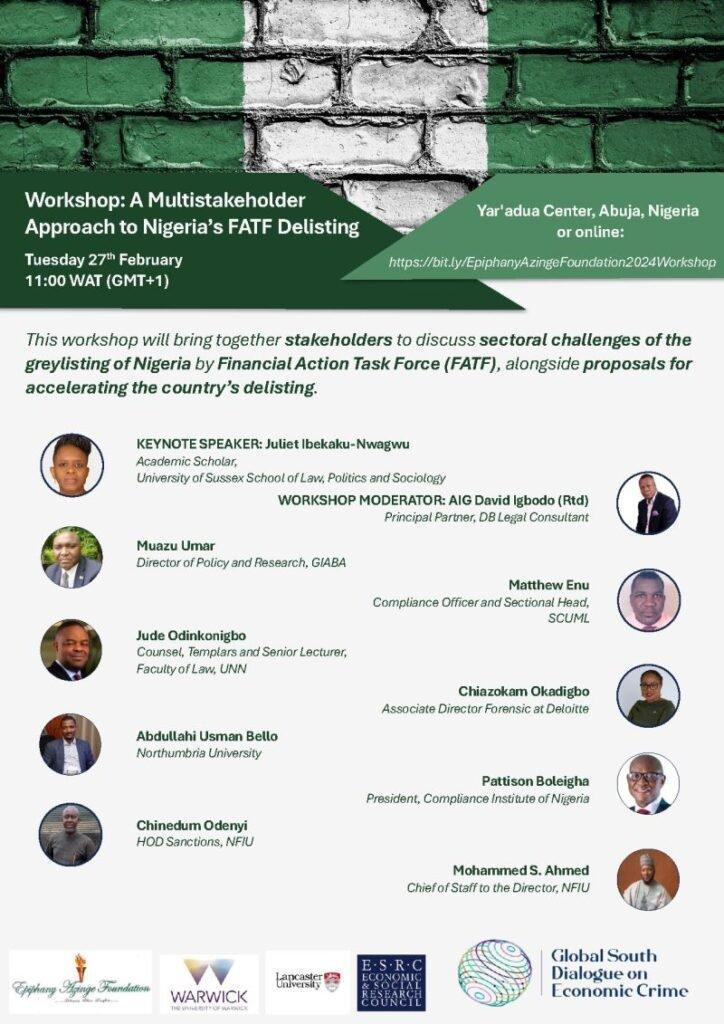
\includegraphics[width=3.125in,height=\textheight,keepaspectratio]{images/strengthen/03_aml.jpg}
\end{center}

\subsection{Publication: Compendium on Lessons Learned from
Anti-Corruption Efforts in Past
Administrations}\label{publication-compendium-on-lessons-learned-from-anti-corruption-efforts-in-past-administrations}

\emph{January 2024}

\href{https://africancenterdev.org/resources/our-publications/compendium/}{A
Compendium on Lessons Learned from Anti-Corruption Efforts in Past
Administrations} (2015-2023) was published to bridge critical knowledge
gaps in Nigeria's governance landscape. This resource documents best
practices, challenges, and strategic insights from nearly a decade of
anti-corruption initiatives.

Providing evidence-based recommendations, the Compendium equips
policymakers, practitioners, civil society organizations, and citizens
with tools to strengthen future anti-corruption efforts. By outlining a
roadmap for reform and practical solutions to governance challenges, it
reinforces the commitment to transparency, accountability, and
institutional integrity.

\begin{center}
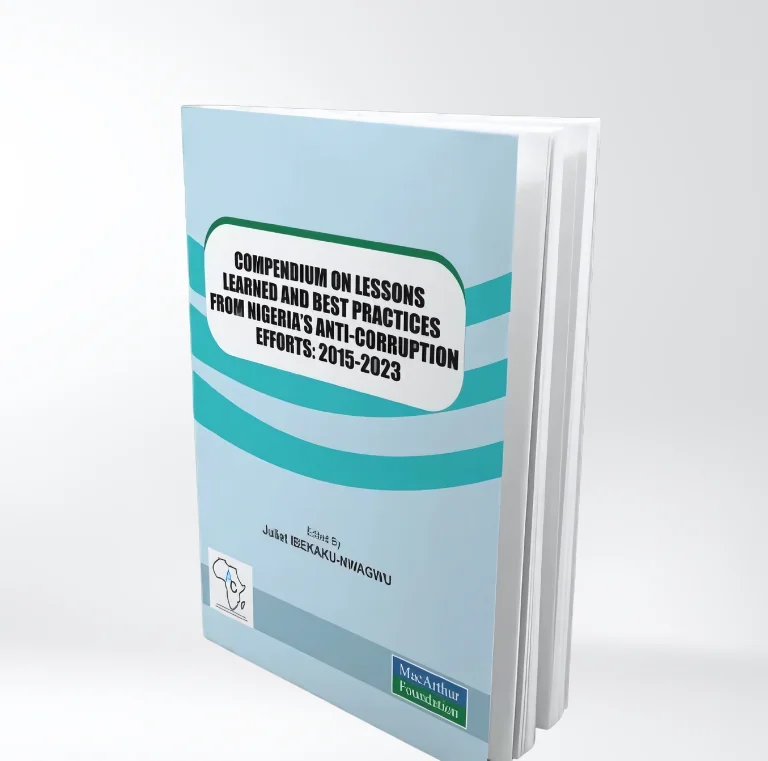
\includegraphics[width=3.125in,height=\textheight,keepaspectratio]{images/strengthen/04_compendium.png}
\end{center}

\subsection{Facilitation: Webinar on the Anti-Money Laundering and
Counter-Financing of Terrorism
Principles}\label{facilitation-webinar-on-the-anti-money-laundering-and-counter-financing-of-terrorism-principles}

The African Center co-hosted a webinar with the NBA Anti-Corruption
Committee on Anti-Money Laundering and Counter-Financing of Terrorism:
Balancing Confidentiality and Compliance. Moderated by Ezenwa Anumnu,
the session examined the new Rules of Professional Conduct (RPC) for
Legal Practitioners in line with FATF standards.

Speakers, including Dr.~Roland Otaru, SAN, and Prof.~Ernest Ojukwu, SAN,
emphasized ethics, Know Your Customer (KYC), record-keeping, and
risk-based reporting. The lead speaker, Juliet Ibekaku-Nwagwu,
highlighted key RPC amendments, legal obligations, and the NBA
Anti-Money Laundering Committee's role in compliance.

With 400 participants, the webinar reinforced the African Center's
commitment to transparency, accountability, and strengthening Nigeria's
efforts to combat money laundering and terrorist financing.

\begin{center}
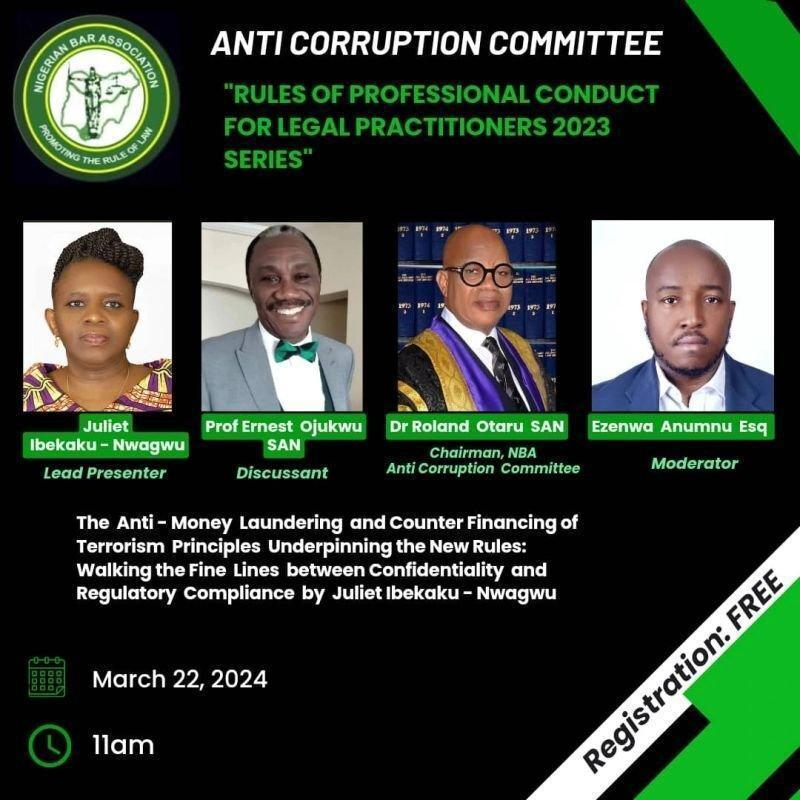
\includegraphics[width=3.125in,height=\textheight,keepaspectratio]{images/strengthen/05_webinar.jpg}
\end{center}

\subsection{Stakeholder Engagement: Review and Implementation Of The
ICRG Action
Plan}\label{stakeholder-engagement-review-and-implementation-of-the-icrg-action-plan}

\emph{June 2024}

In partnership with GSDEC, we convened key stakeholders to accelerate
Nigeria's removal from the FATF grey list. With support from the
Economic and Social Research Council (ESRC), the session focused on
urgent actions and collective responsibility in achieving this goal.

Senior officials from NFIU, EFCC, NDLEA, and FMOJ outlined Nigeria's
progress since its 2023 greylisting, highlighting strengthened laws,
enhanced money laundering prosecutions, and improved international
cooperation.

Reaffirming their commitment, stakeholders pledged to drive strategic
reforms, enhance asset recovery efforts, and bolster AML/CFT
enforcement, ensuring Nigeria's swift and lasting compliance.

\begin{figure}

\begin{minipage}{0.47\linewidth}
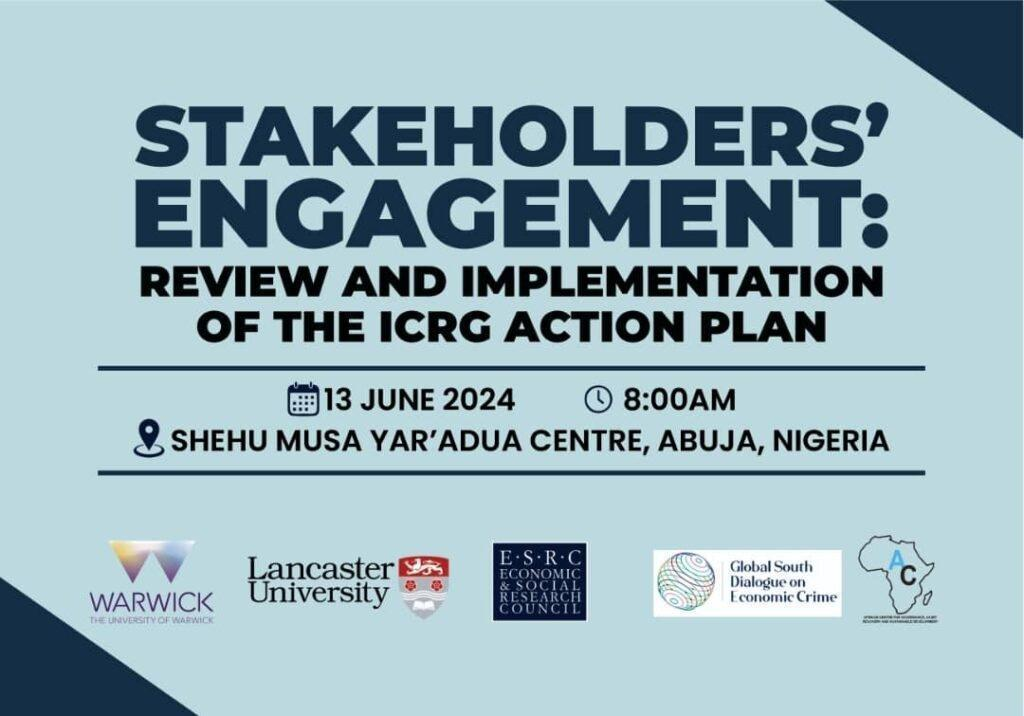
\includegraphics[width=3.64583in,height=\textheight,keepaspectratio]{images/strengthen/06_0_stake.jpg}\end{minipage}%
%
\begin{minipage}{0.53\linewidth}
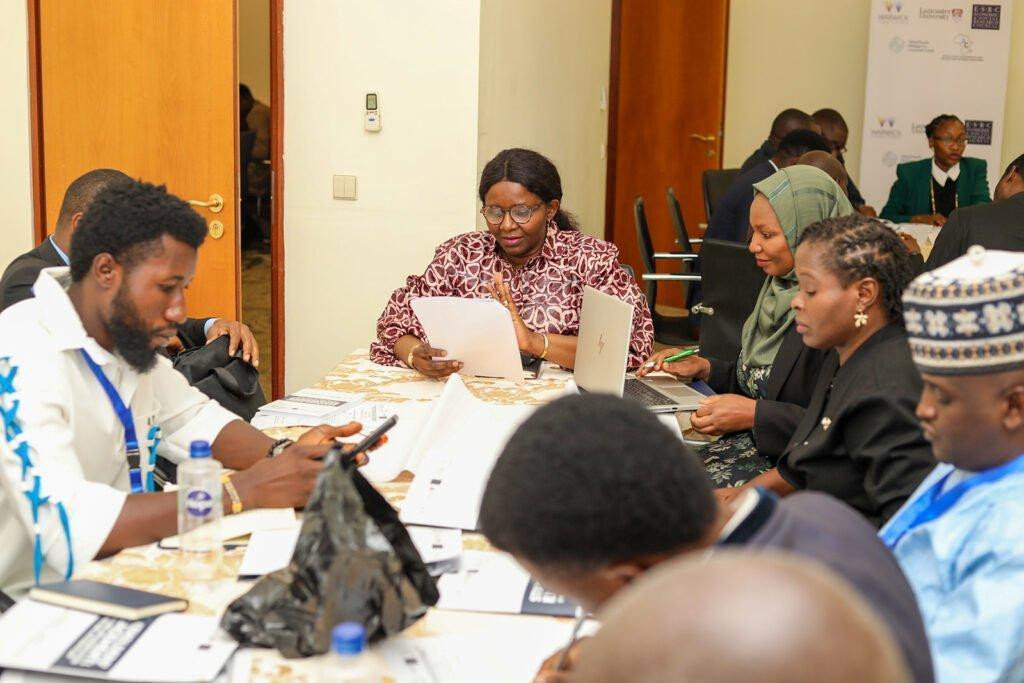
\includegraphics[width=4.16667in,height=\textheight,keepaspectratio]{images/strengthen/06_1_stake.jpg}\end{minipage}%

\end{figure}%

\subsection{Training: Nigerian Investigative Journalists Workshop in
Collaboration with RUSI,
UK}\label{training-nigerian-investigative-journalists-workshop-in-collaboration-with-rusi-uk}

In partnership with RUSI, we hosted a webinar Demystifying FATF to equip
investigative journalists with the tools to combat corruption. The
session provided a deep dive into FATF's processes, its role in
promoting financial integrity, and how journalists can leverage this
knowledge in their work.

Discussions also explored Nigeria's recent Mutual Evaluation Report
(MER), highlighting the implications of the country's greylisting. By
empowering investigative journalists with critical expertise, the
African Center reinforces its commitment to fostering transparency,
accountability, and a stronger financial system in Nigeria.

\begin{center}
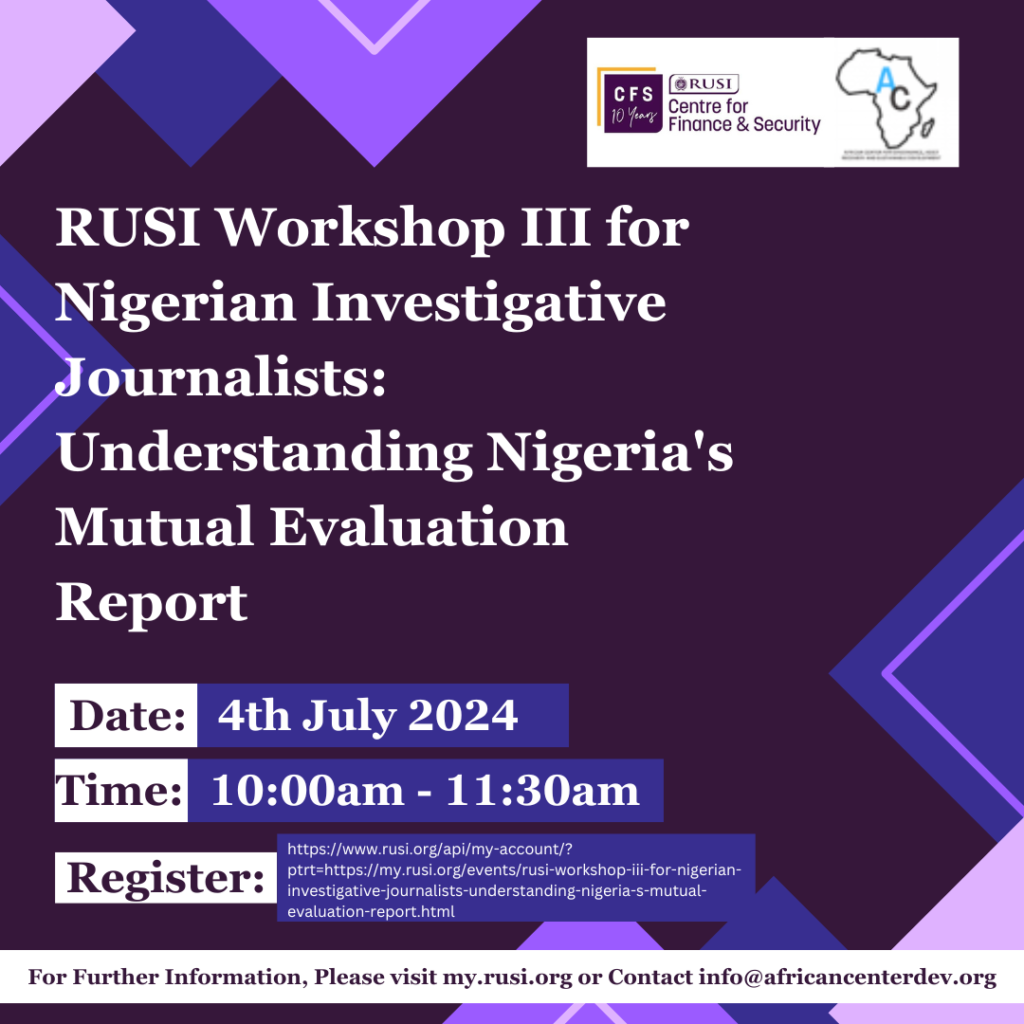
\includegraphics[width=3.125in,height=\textheight,keepaspectratio]{images/strengthen/07_rusi.png}
\end{center}

\subsection{Participation: International Anti-Corruption
Conference}\label{participation-international-anti-corruption-conference}

The African Center for Governance reaffirmed its commitment to combating
corruption by actively participating in the International
Anti-Corruption Conference (IACC) 2024. Engaging with global leaders,
policymakers, and civil society organizations, the Center strengthened
partnerships and fostered new collaborations.

Key sessions addressed critical issues such as global threats to
integrity, business ethics, technology's role in anti-corruption, and
the impact of corruption on human rights and democracy. The African
Center also participated in the CSO session with the MacArthur
Foundation, providing updates on Nigeria's anti-corruption efforts.

Through its participation, the African Center reinforced its role as a
leading voice in promoting transparency, accountability, and strong
institutions across Africa.

\begin{figure}

\begin{minipage}{0.38\linewidth}
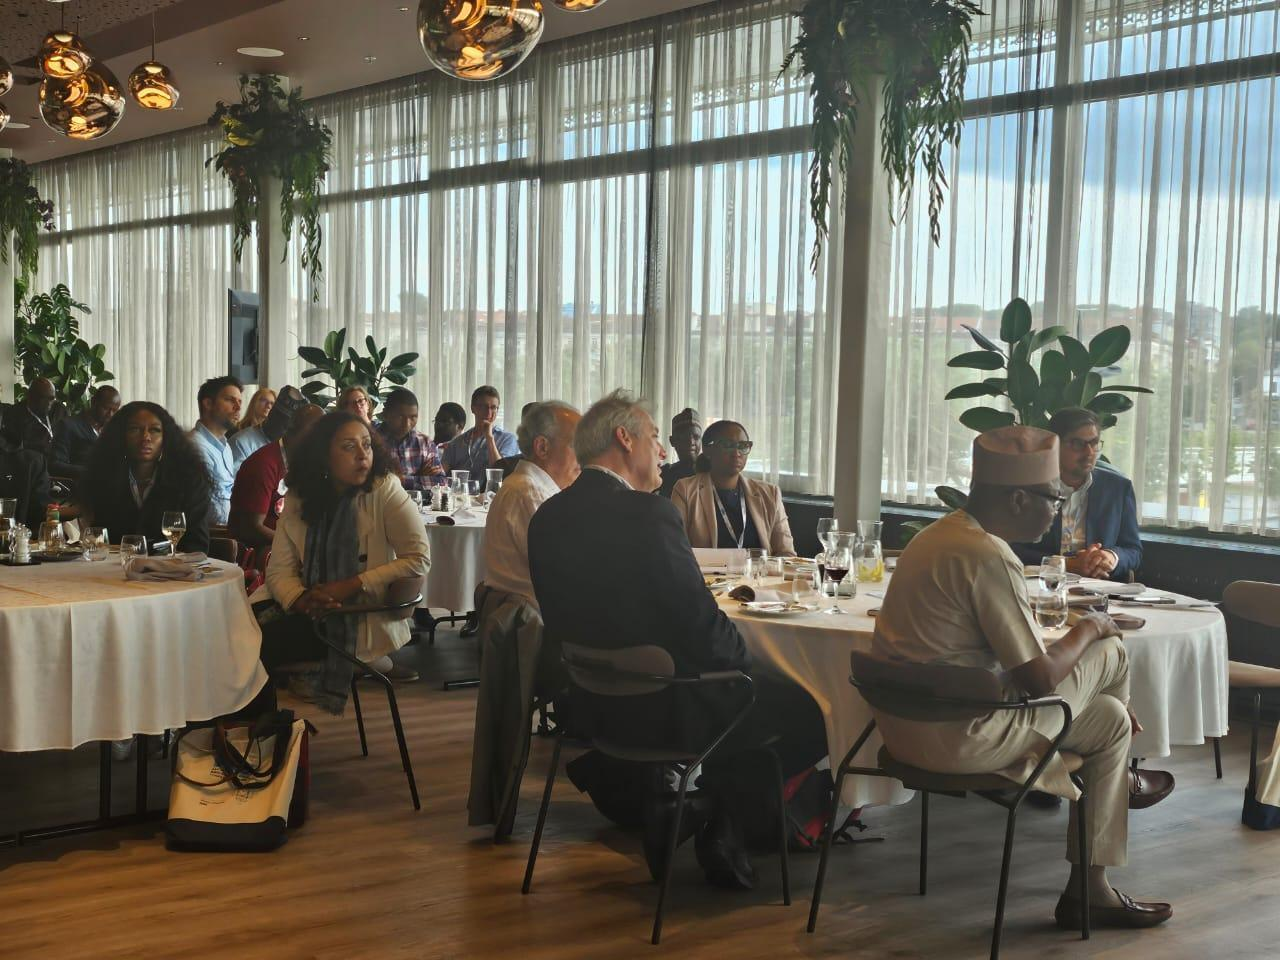
\includegraphics[width=3.125in,height=\textheight,keepaspectratio]{images/strengthen/08_0_acc.jpg}\end{minipage}%
%
\begin{minipage}{0.25\linewidth}
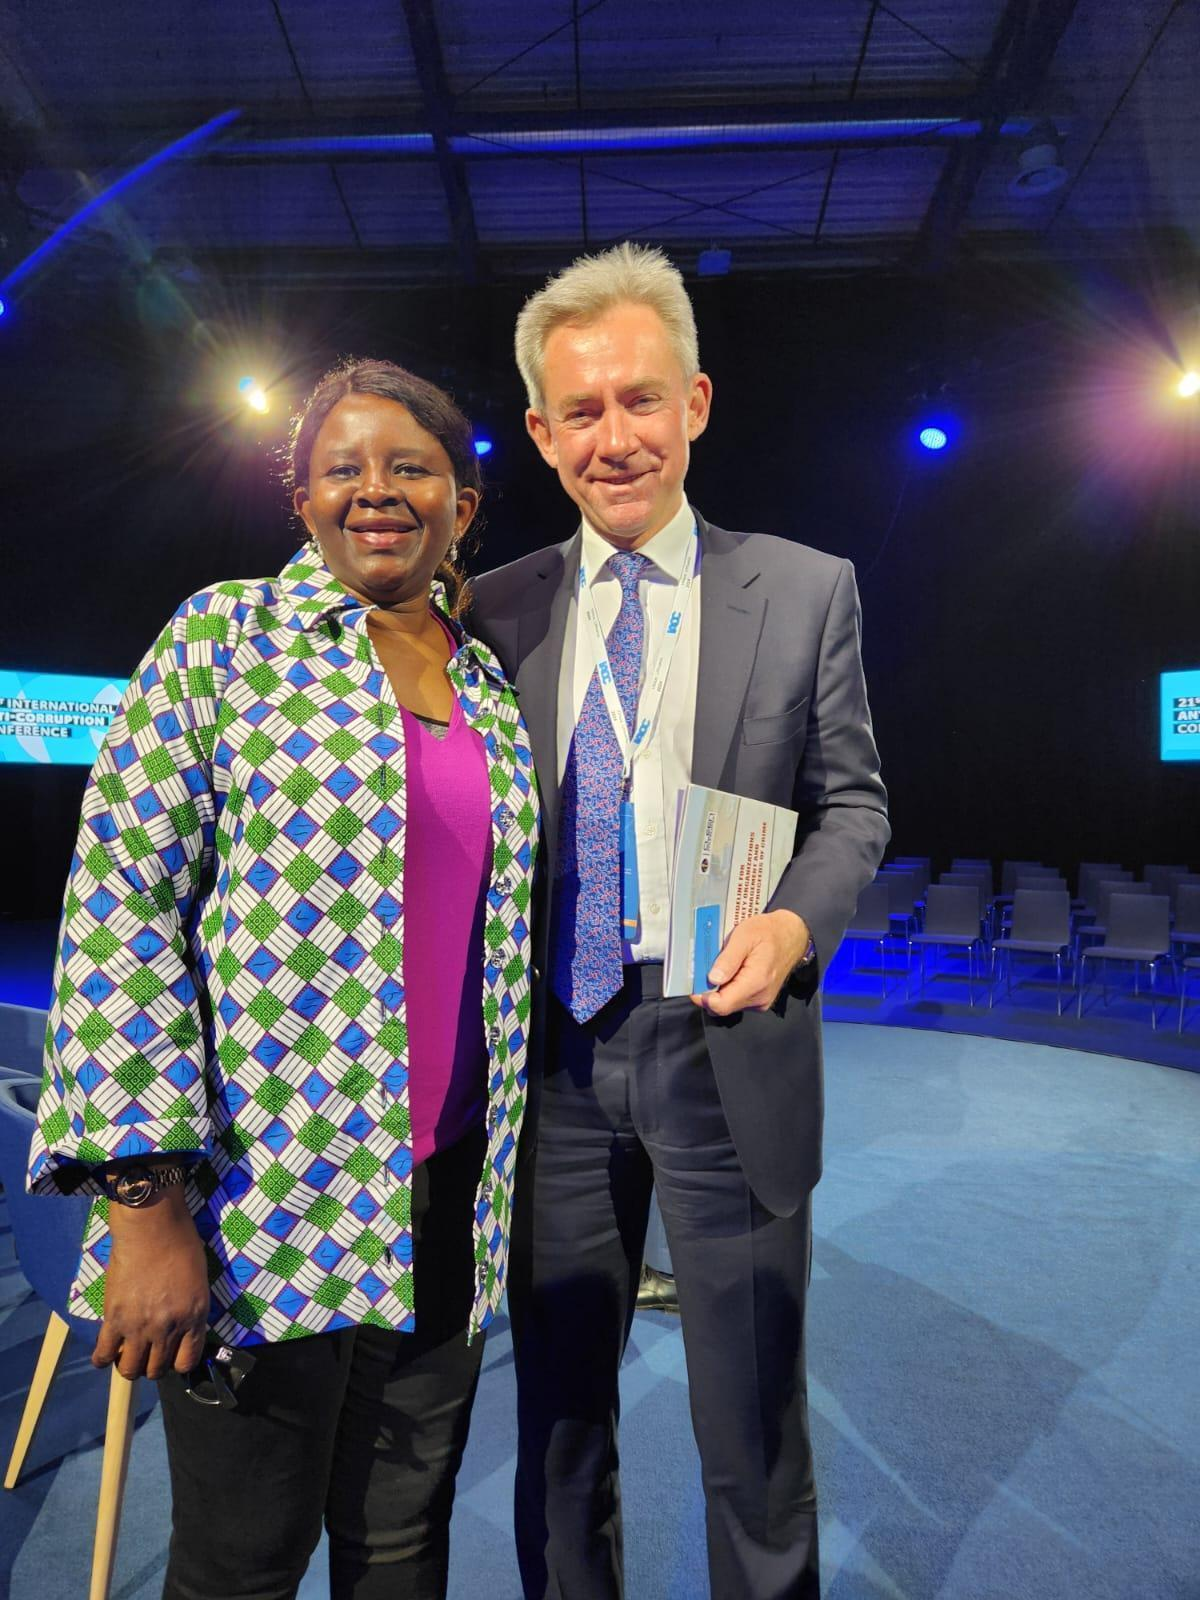
\includegraphics[width=2.08333in,height=\textheight,keepaspectratio]{images/strengthen/08_2_acc.jpg}\end{minipage}%
%
\begin{minipage}{0.38\linewidth}
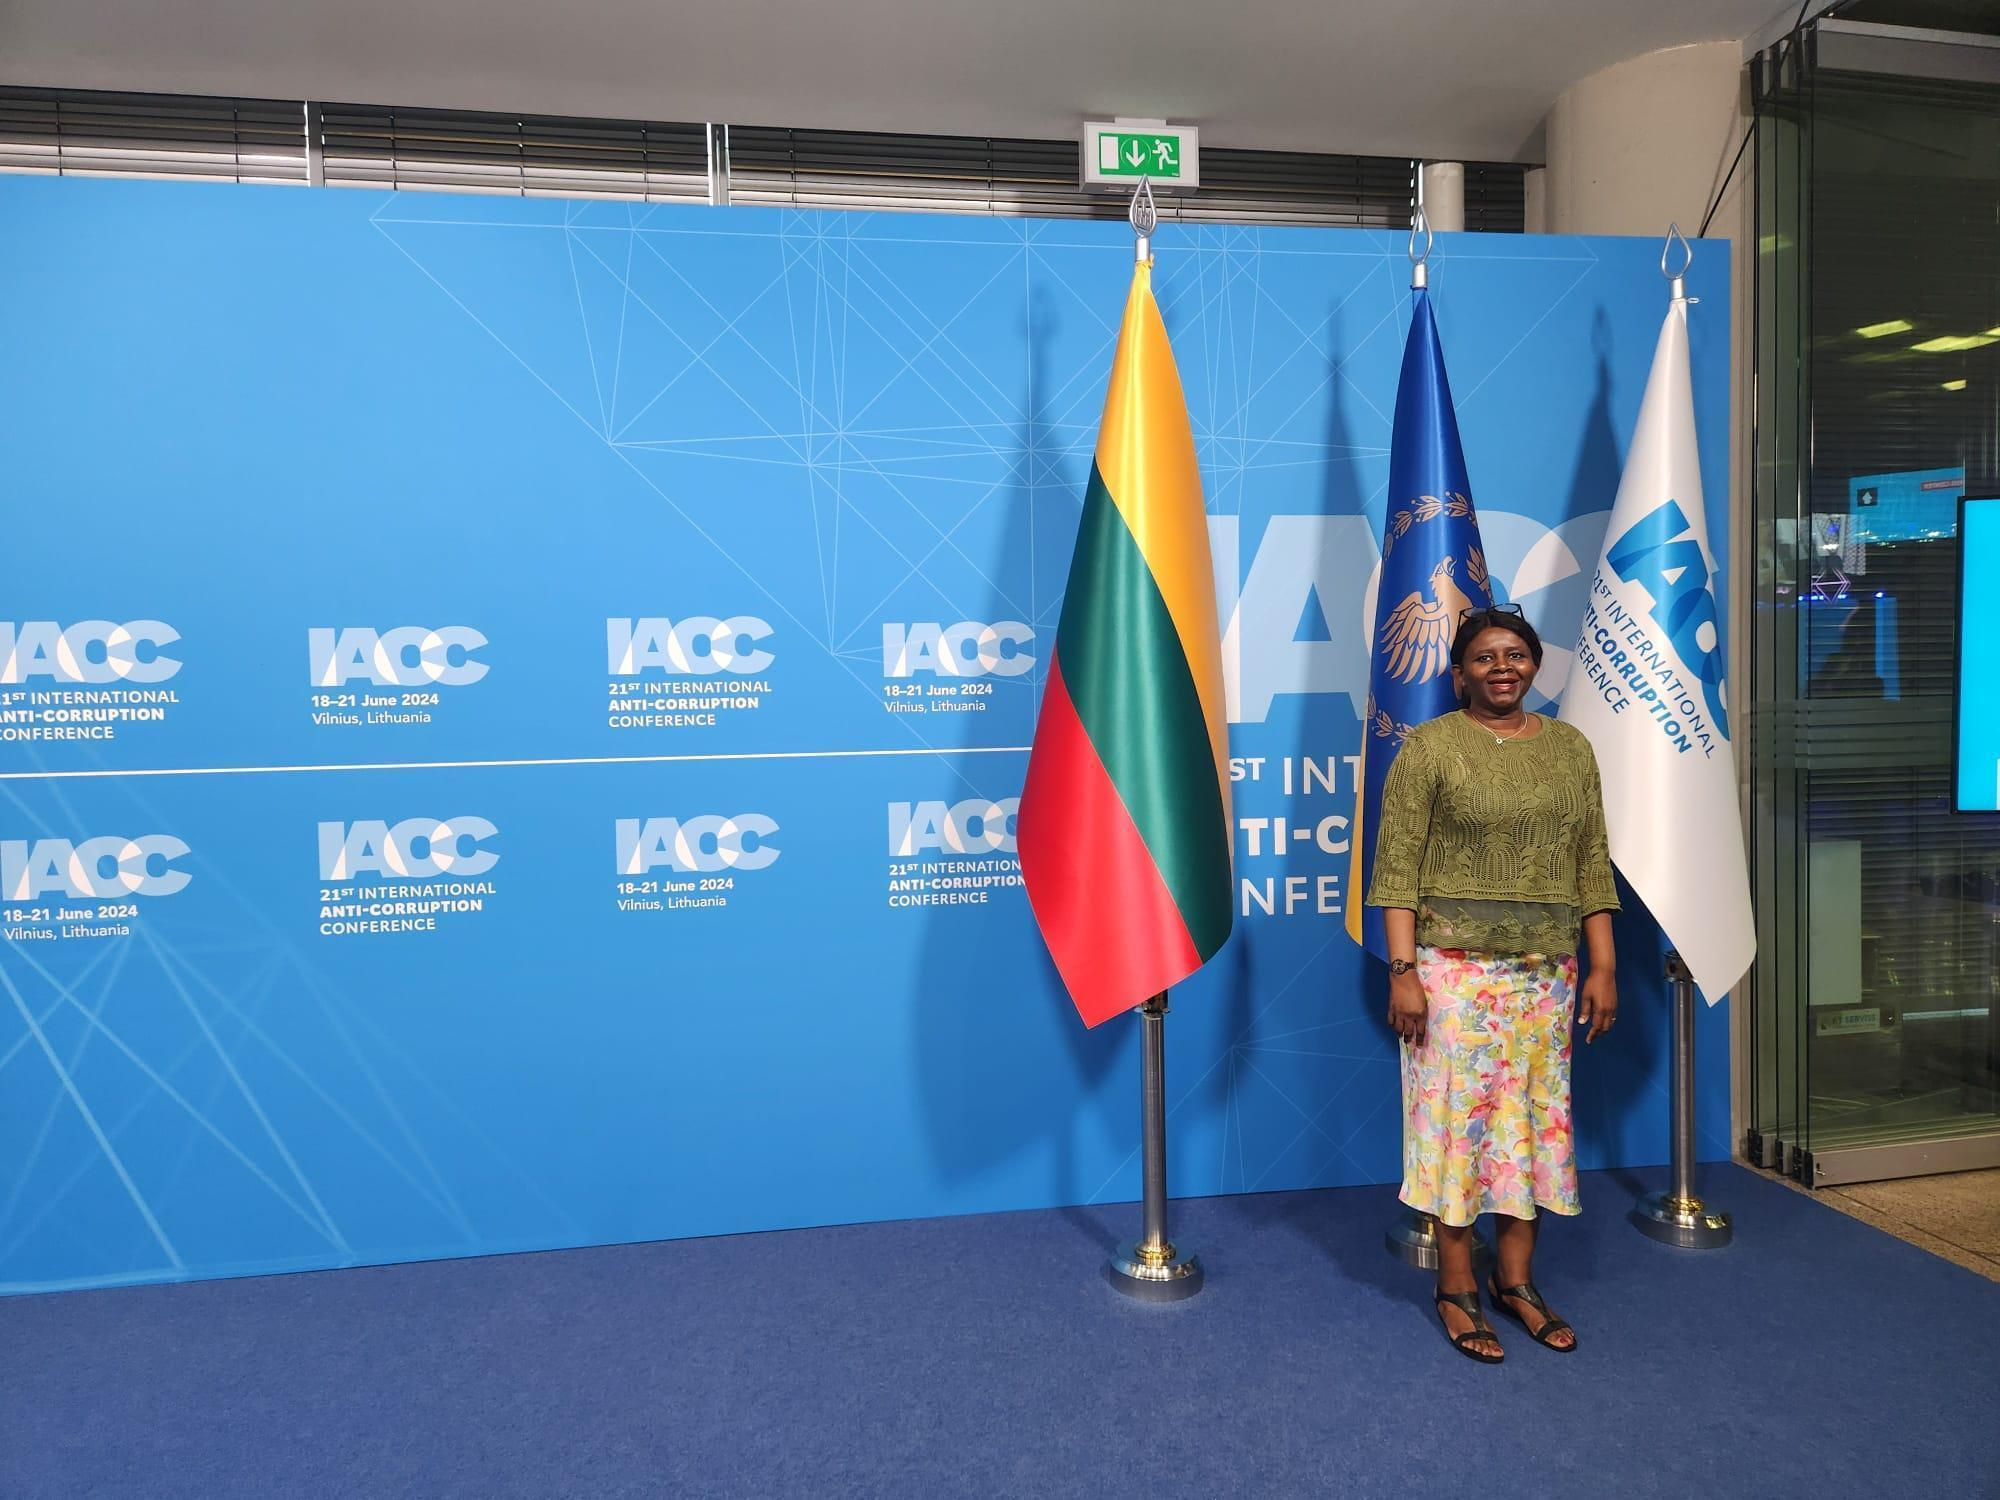
\includegraphics[width=3.125in,height=\textheight,keepaspectratio]{images/strengthen/08_1_acc.jpg}\end{minipage}%

\end{figure}%

\subsection{Presentation: ``An Overview of Corruption in the Oil Sector
in Nigeria'' at HEDA Resource
CenterConference}\label{presentation-an-overview-of-corruption-in-the-oil-sector-in-nigeria-at-heda-resource-centerconference}

The African Center participated in the HEDA Resource Center's first
International Anti-Corruption \& Climate Change Conference. Contributing
to the panel on ``Corruption in the Oil Sector,'' the discussion focused
on major cases such as OPL245, P\&ID, and Glencore, highlighting their
impact on anti-corruption efforts. The session featured key
stakeholders, including representatives from ANEEJ, EFCC, and the Kano
Anti-Corruption Commission.

\begin{center}
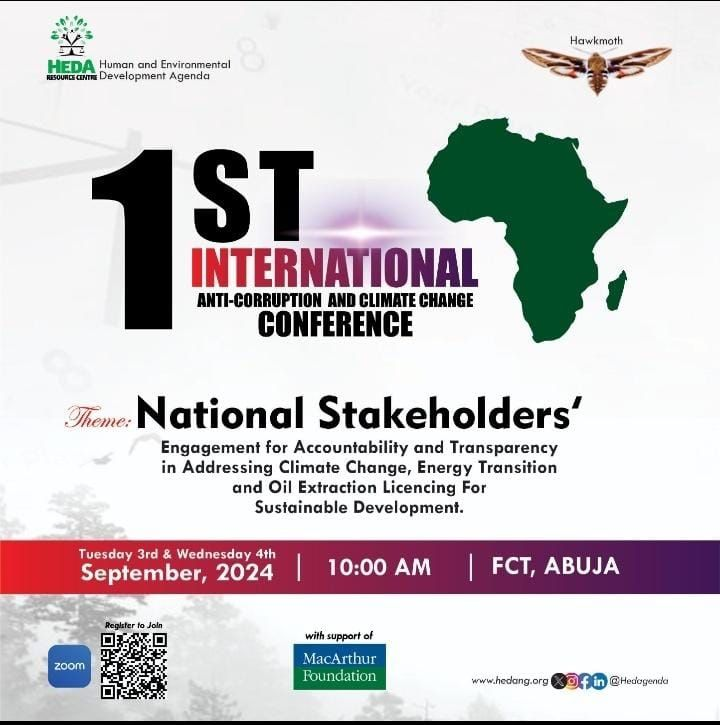
\includegraphics[width=3.125in,height=\textheight,keepaspectratio]{images/strengthen/09_oil.png}
\end{center}

\subsection{Participation: UNCAC Implementation Review
Group}\label{participation-uncac-implementation-review-group}

\emph{September 2024}

The first part of the resumed Fifteenth Session assessed the
implementation of the United Nations Convention against Corruption,
focusing on Chapters II (Preventive Measures) and III (Criminalization
and Law Enforcement). Established under Resolution 3/1, the
Implementation Review Group serves as an open-ended intergovernmental
body, overseeing the review process, identifying challenges and best
practices, and addressing technical assistance needs to enhance the
Convention's effectiveness.

\begin{center}
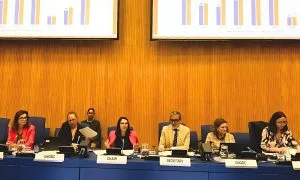
\includegraphics[width=3.64583in,height=\textheight,keepaspectratio]{images/strengthen/10_uncac.png}
\end{center}

\subsection{Launch: Guidelines for Civil Society Organizations on
Managing and Monitoring Proceeds of Crime in
Nigeria}\label{launch-guidelines-for-civil-society-organizations-on-managing-and-monitoring-proceeds-of-crime-in-nigeria}

In partnership with CLEEN Foundation, we presented the Guidelines for
Civil Society Organizations (CSOs) on Monitoring and Managing Proceeds
of Crime, emphasizing CSO involvement in asset recovery. Key
stakeholders from the Federal Ministry of Justice, ICPC, NBA, and over
sixty CSOs discussed legal frameworks like UNCAC, AUCPCC, and Nigeria's
Proceeds of Crime Act (2022), highlighting CSOs' role in promoting
accountability.

Participants called for stronger legal provisions to empower citizens in
asset recovery. The African Center and CLEEN Foundation were recognized
for fostering collaboration between state and non-state actors to
enhance transparency and sustainable development.

\begin{figure}

\begin{minipage}{0.40\linewidth}
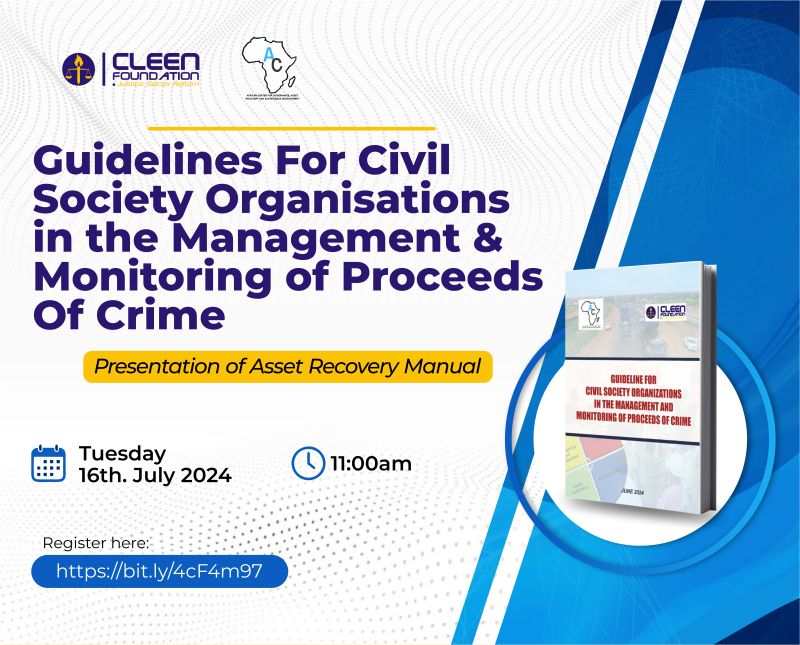
\includegraphics[width=3.125in,height=\textheight,keepaspectratio]{images/strengthen/11_0_guide.png}\end{minipage}%
%
\begin{minipage}{0.60\linewidth}
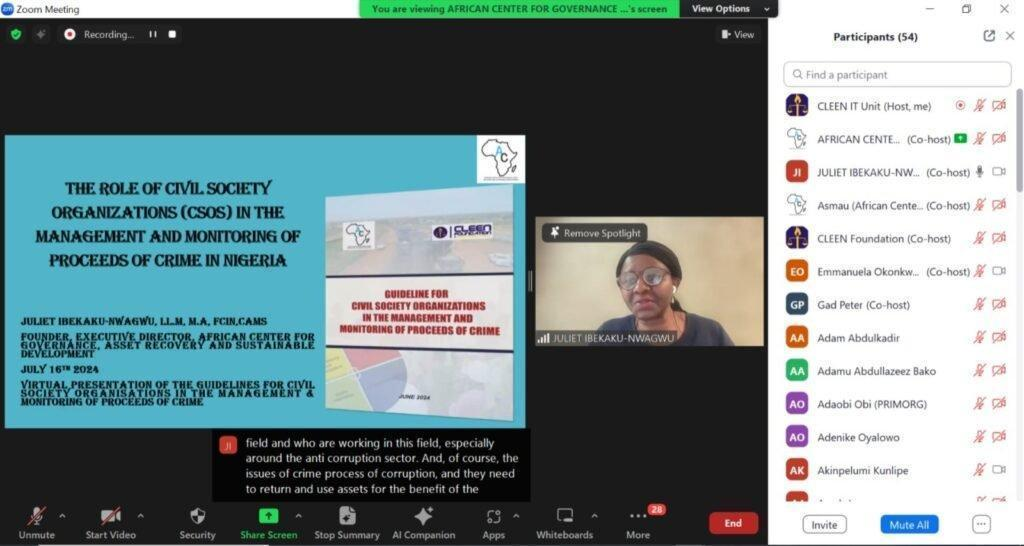
\includegraphics[width=4.6875in,height=\textheight,keepaspectratio]{images/strengthen/11_1_guide.jpg}\end{minipage}%

\end{figure}%

\subsection{Facilitation: African Development Bank 2024 Anti-Corruption
Seminar}\label{facilitation-african-development-bank-2024-anti-corruption-seminar}

The 2024 Anti-Corruption Seminar, themed ``Profit from Integrity:
Capitalizing on Anti-Corruption Measures in Africa,'' brought together
esteemed experts to tackle corruption in Africa. The seminar emphasized
the significance of asset recovery in deterring criminals, restoring
justice, and promoting sustainable development.

Emphasizing the need for diplomatic engagement and collective action,
speakers noted that asset recovery extends beyond legal measures. The
session called for a review of the Common African Position on Asset
Recovery (CAPAR) and the AUCPCC to assess progress toward the UN
Sustainable Development Goals and the African Union's Agenda 2063.

\begin{figure}

\begin{minipage}{0.39\linewidth}
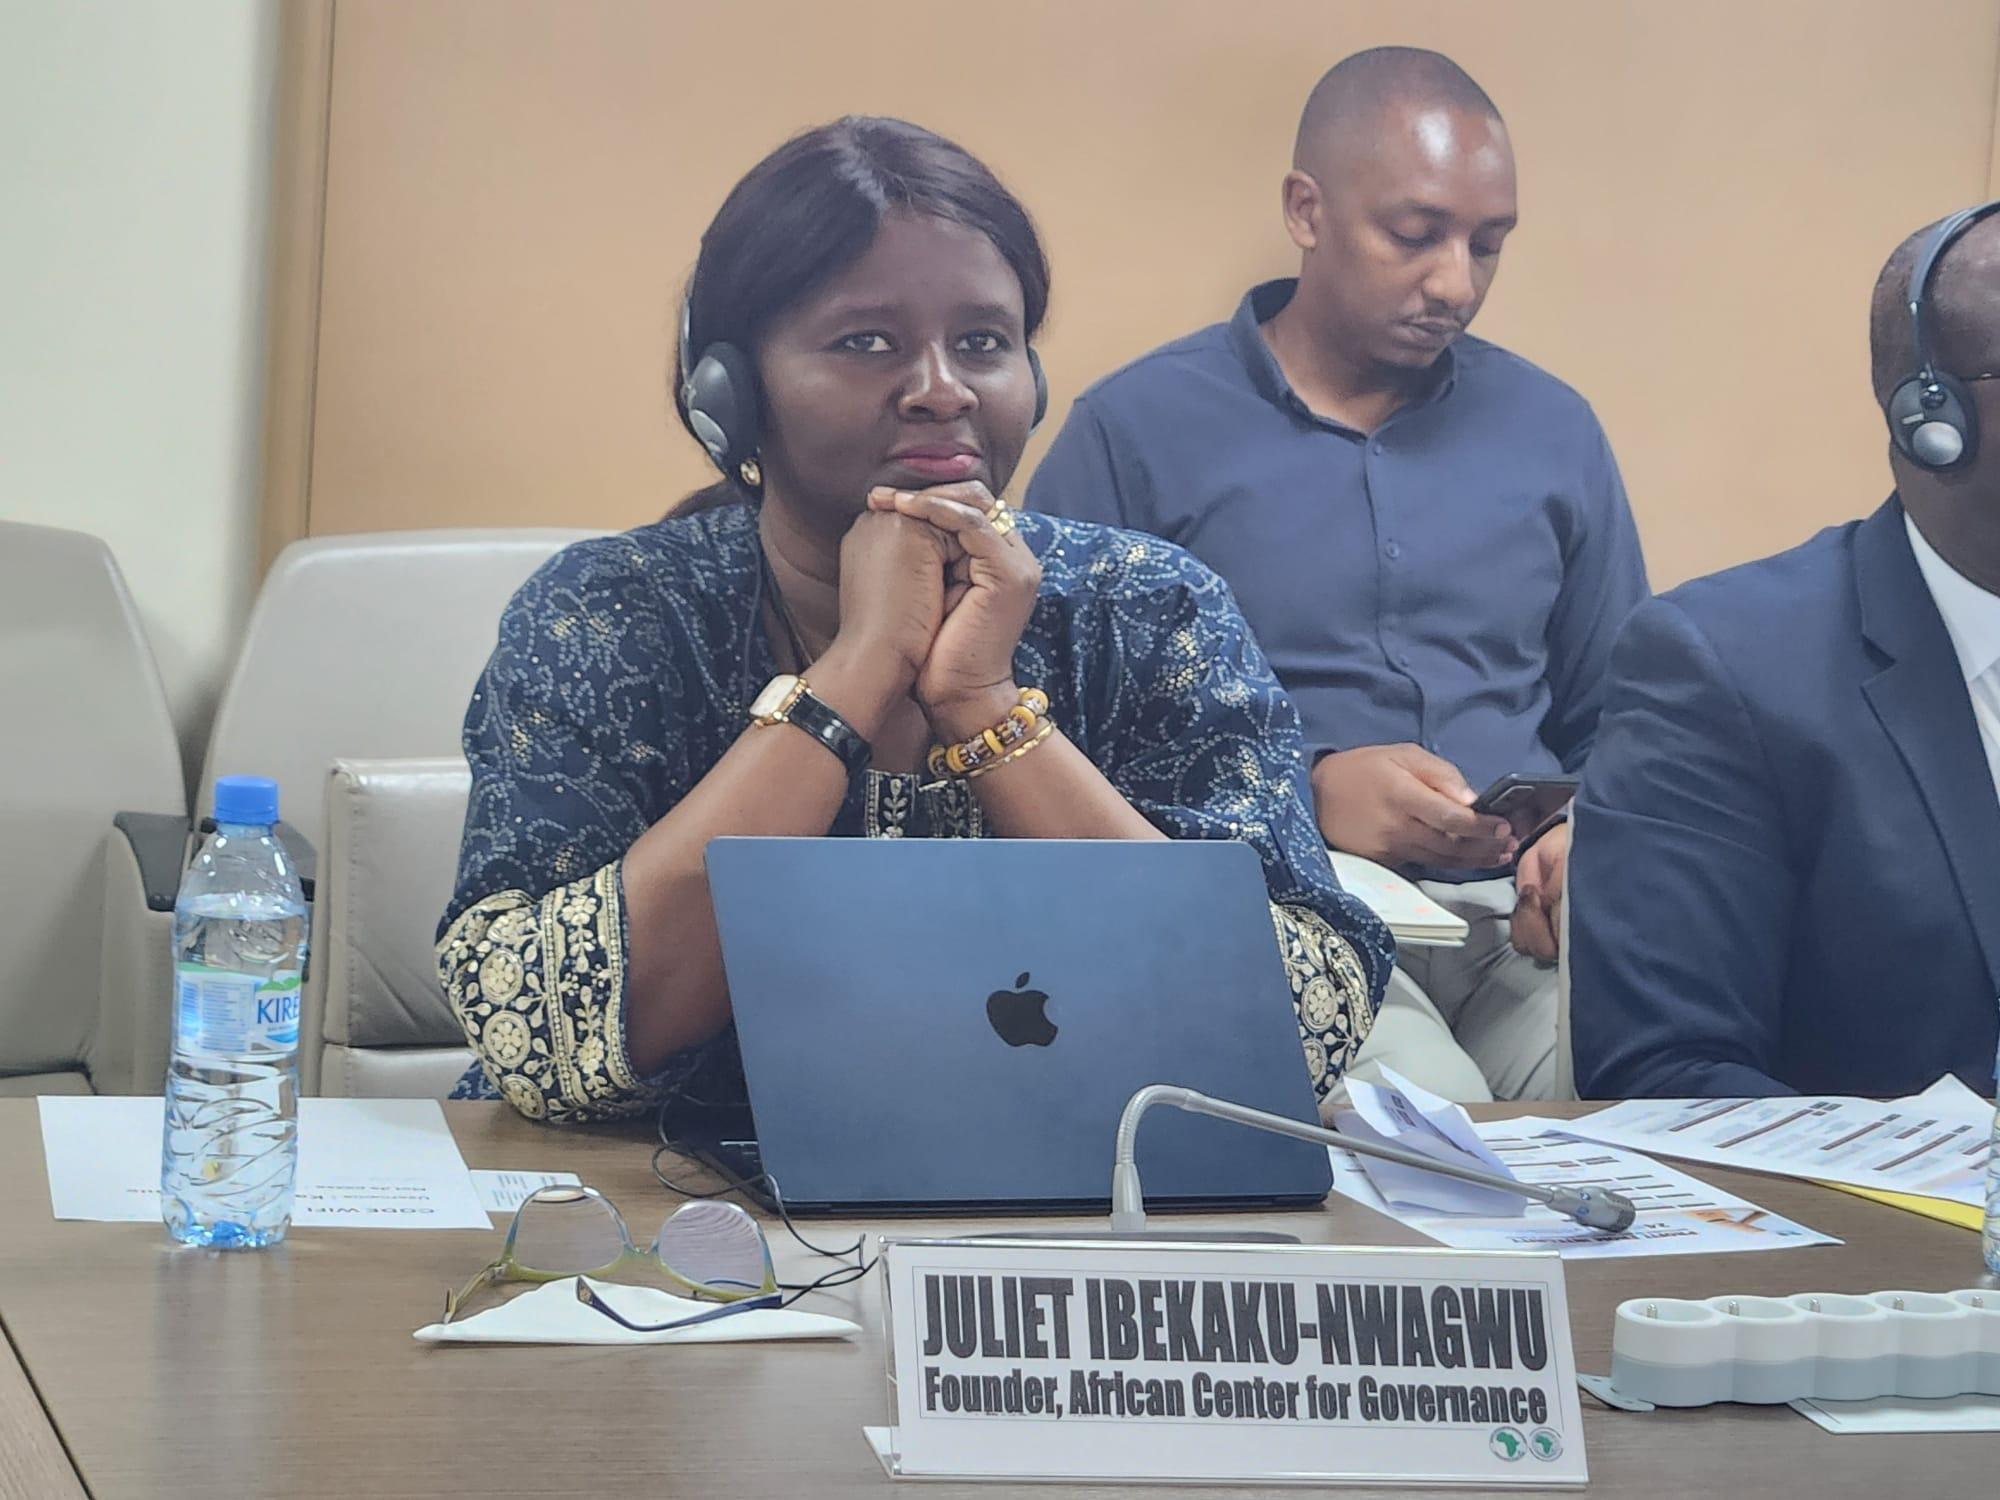
\includegraphics[width=2.60417in,height=\textheight,keepaspectratio]{images/strengthen/12_0_afdb.jpg}\end{minipage}%
%
\begin{minipage}{0.61\linewidth}
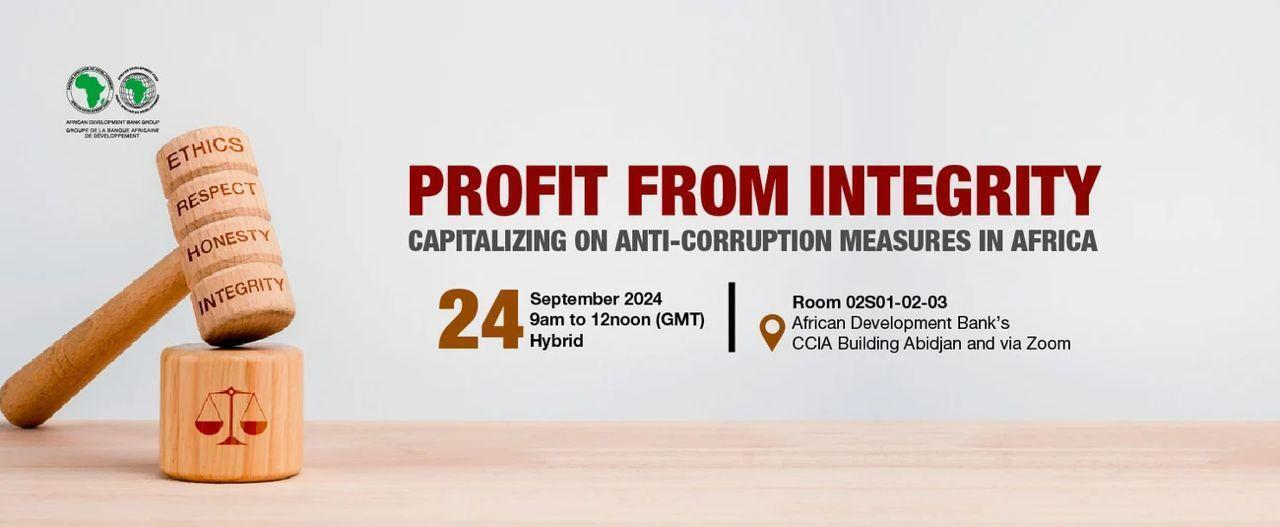
\includegraphics[width=4.16667in,height=\textheight,keepaspectratio]{images/strengthen/12_1_afdb.jpg}\end{minipage}%

\end{figure}%

\subsection{Facilitation: Event on Combating Illicit Financial Flows in
Africa's Extractive Sector at the UNTOC Conference of
Parties}\label{facilitation-event-on-combating-illicit-financial-flows-in-africas-extractive-sector-at-the-untoc-conference-of-parties}

The African Center hosted a panel on Countering Illicit Financial Flows
(IFFs) in the Extractive Industry during the 12th UNTOC Conference of
Parties. Moderated by Brook Horowitz, CEO of IBLF Global, the discussion
examined strategies to curb IFFs and drive sustainable development in
Africa.

Experts highlighted Nigeria's extractive sector as a major contributor
to Africa's IFFs, citing discretionary licensing as a key driver. The
session emphasized strengthening asset recovery, enforcing anti-money
laundering standards, adopting UN COSP Resolution 10/23 on Beneficial
Ownership, and sanctioning financial secrecy jurisdictions to combat
illicit flows.

\begin{figure}

\begin{minipage}{0.50\linewidth}
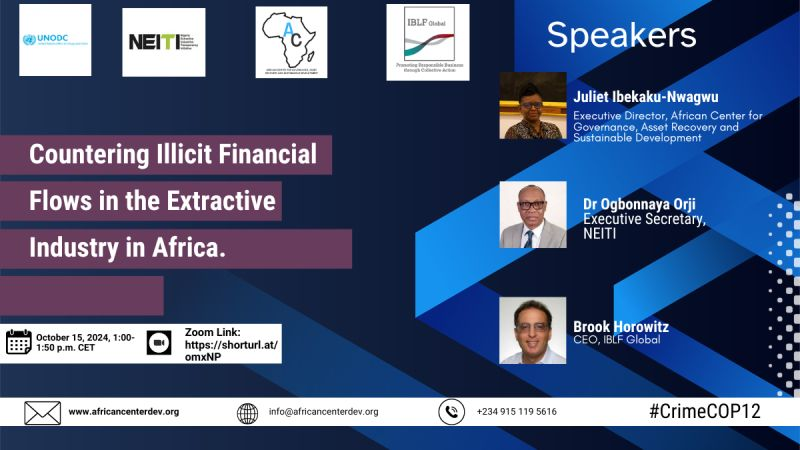
\includegraphics[width=3.125in,height=\textheight,keepaspectratio]{images/strengthen/13_0_iff.png}\end{minipage}%
%
\begin{minipage}{0.50\linewidth}
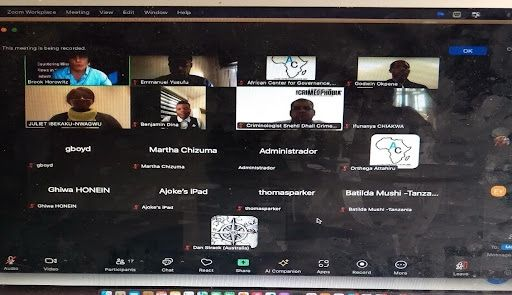
\includegraphics[width=3.125in,height=\textheight,keepaspectratio]{images/strengthen/13_1_iff.png}\end{minipage}%

\end{figure}%

\subsection{Facilitation: Risk Assessment Workshops across
Nigeria}\label{facilitation-risk-assessment-workshops-across-nigeria}

In collaboration with the NBA, the NBA Anti-Money Laundering Committee
(NBA-AMLC) we held the AML/CFT Legal Sector Risk Assessment Workshops in
Lagos, Abuja, Yola, Port Harcourt, Kano, and Enugu to strengthen
lawyers' ability to combat financial crime through a risk based
assessment of possible ML/FT/PF risks. The workshop assessed ML/FT/PF
risks through online questionnaires and in-person sessions from October
28 to 31.

Engaging 375 legal professionals, key stakeholders, and regulators, the
workshop fostered dialogue on risk assessment and compliance. At the
Abuja session on December 31, 2024, NBA President Mazi Afam Osigwe SAN
emphasized balancing client confidentiality with preventing legal
services misuse for illicit activities.

\begin{figure}

\begin{minipage}{0.50\linewidth}
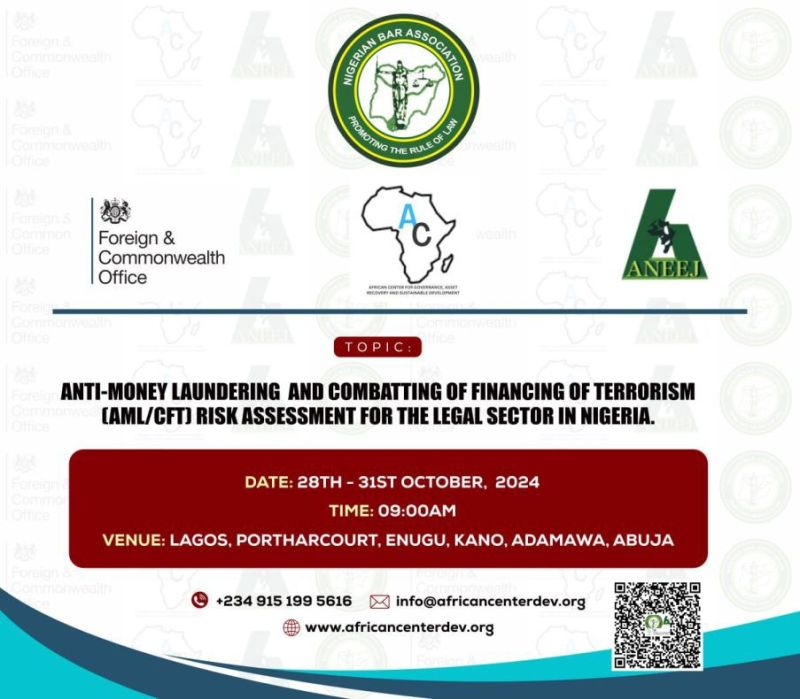
\includegraphics[width=3.64583in,height=\textheight,keepaspectratio]{images/strengthen/14_0_risk.png}\end{minipage}%
%
\begin{minipage}{0.50\linewidth}
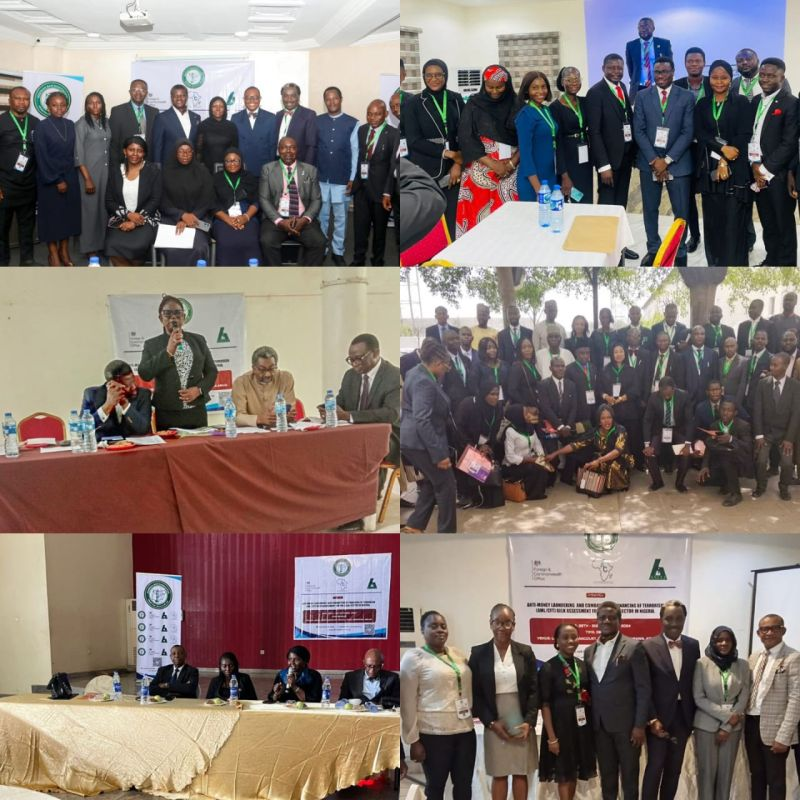
\includegraphics[width=3.64583in,height=\textheight,keepaspectratio]{images/strengthen/14_1_risk.png}\end{minipage}%

\end{figure}%

\subsection{Facilitation: Validation and Joint Action Planning Meeting
for the
NBA-AMLC}\label{facilitation-validation-and-joint-action-planning-meeting-for-the-nba-amlc}

The African Center collaborated with the NBA Anti-Money Laundering
Committee (NBA-AMLC) in a strategic session to address money laundering
and illicit financial flows. The session reviewed findings from the
recently developed Risk Assessment Report for Legal Sector and explored
measures to enhance compliance in the legal sector. Key presentations
outlined challenges and proposed reforms, reinforcing the commitment to
financial integrity and accountability.

\begin{figure}

\begin{minipage}{0.33\linewidth}
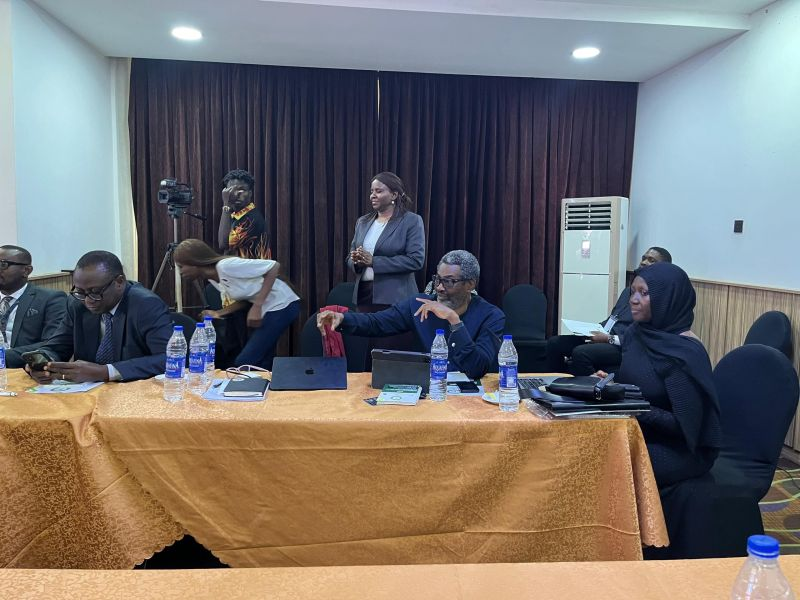
\includegraphics[width=3.64583in,height=\textheight,keepaspectratio]{images/strengthen/15_1_nba.png}\end{minipage}%
%
\begin{minipage}{0.33\linewidth}
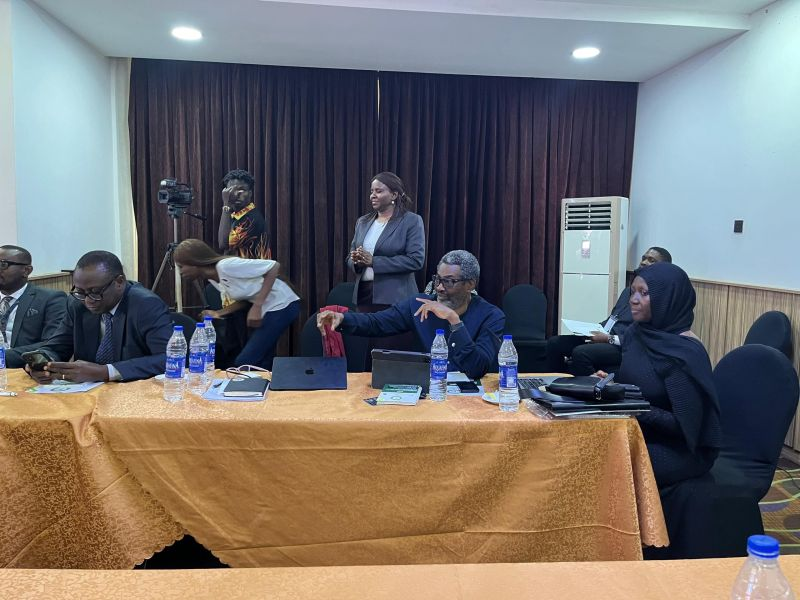
\includegraphics[width=3.64583in,height=\textheight,keepaspectratio]{images/strengthen/15_1_nba.png}\end{minipage}%
%
\begin{minipage}{0.33\linewidth}
\includegraphics[width=3.64583in,height=\textheight,keepaspectratio]{images/strengthen/15_2_nba.png}\end{minipage}%

\end{figure}%

\subsection{Training: NBA Executives}\label{training-nba-executives}

In collaboration with the NBA Anti-Money Laundering Committee (NBA-AMLC)
and ANEEJ, we hosted a Hybrid Training Program for NBA Branch Executive
Chairmen to enhance compliance and ethical leadership in the legal
sector. The training covered the Rules of Professional Conduct (RPC),
key findings from the Risk Assessment Report (RAR), and strategies to
mitigate money laundering risks. A key highlight was the unveiling of
the AML/CFT Legal Sector Risk Assessment Report, reinforcing the NBA's
commitment to strengthening Nigeria's legal framework and aligning with
global anti-financial crime standards.

\begin{figure}

\begin{minipage}{0.31\linewidth}
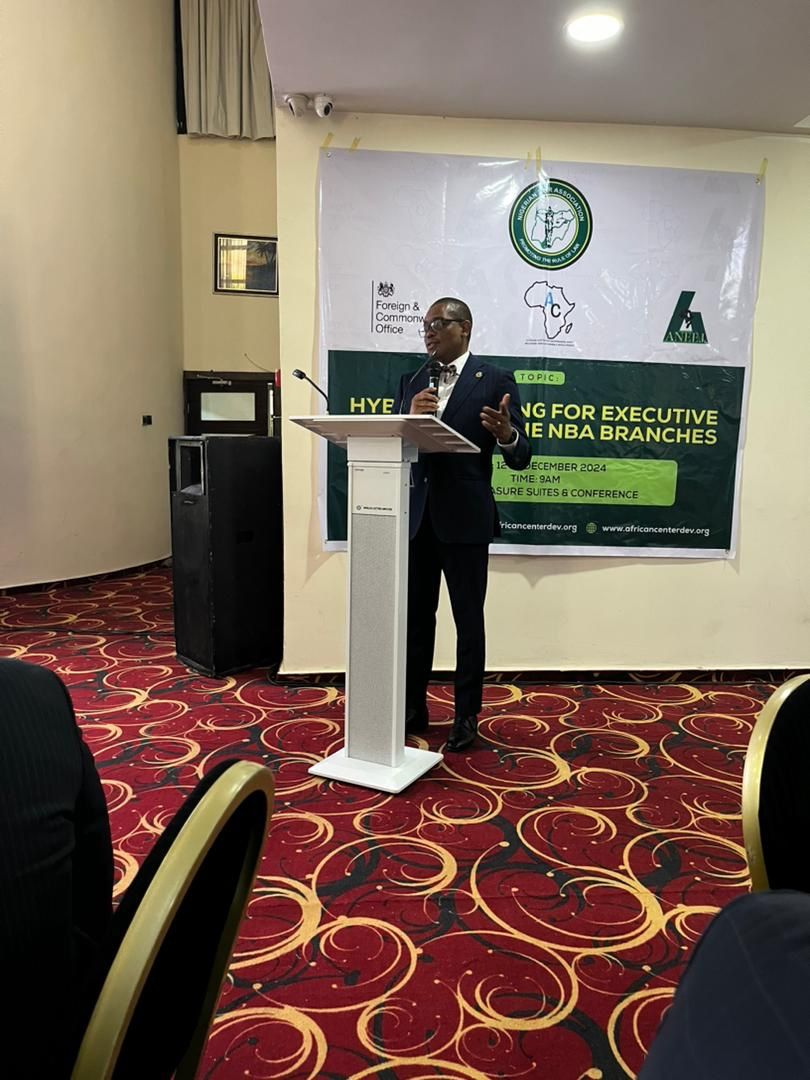
\includegraphics[width=2.08333in,height=\textheight,keepaspectratio]{images/strengthen/16_0_hnba.png}\end{minipage}%
%
\begin{minipage}{0.69\linewidth}
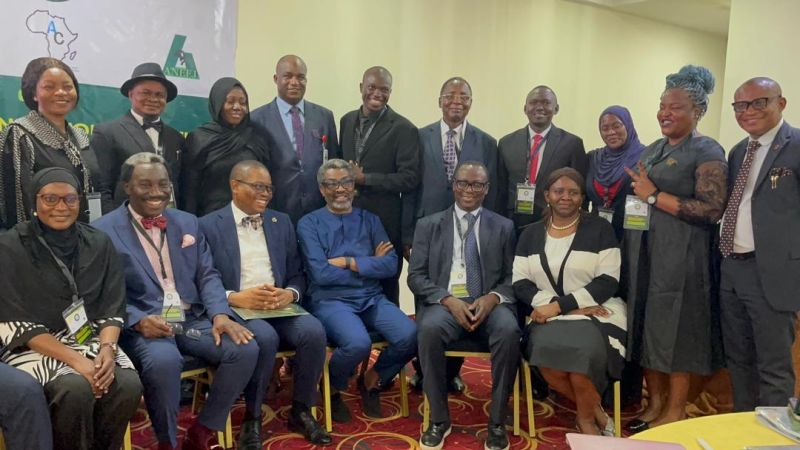
\includegraphics[width=4.6875in,height=\textheight,keepaspectratio]{images/strengthen/16_1_hnba.png}\end{minipage}%

\end{figure}%

\subsection{Publication: Risk Assessment Report for the Legal Sector in
Nigeria}\label{publication-risk-assessment-report-for-the-legal-sector-in-nigeria}

Nigeria's mutual evaluation reports and recent case studies have
demonstrated the vulnerabilities of legal professionals to ML/TF/PF. In
response, the Nigerian Bar Association Anti-Money Laundering Committee
(NBA-AMLC) conducted a risk assessment survey. The scope of the survey
was to gain a strong understanding of the AML/CFT/PF vulnerabilities
that legal professionals perceive themselves to be exposed to, evaluate
the level of knowledge, awareness, and training that lawyers have in
relation to AML/CFT/PF compliance. The
\href{https://africancenterdev.org/nba-legal-sector-risk-assessment-report-2024}{Risk
Assessment Report} represents a significant step towards enhancing the
legal sector's compliance with Nigeria's Anti-Money Laundering,
Counter-Terrorist Financing, and Proliferation Financing (AML/CFT/PF)
obligations.

\begin{center}
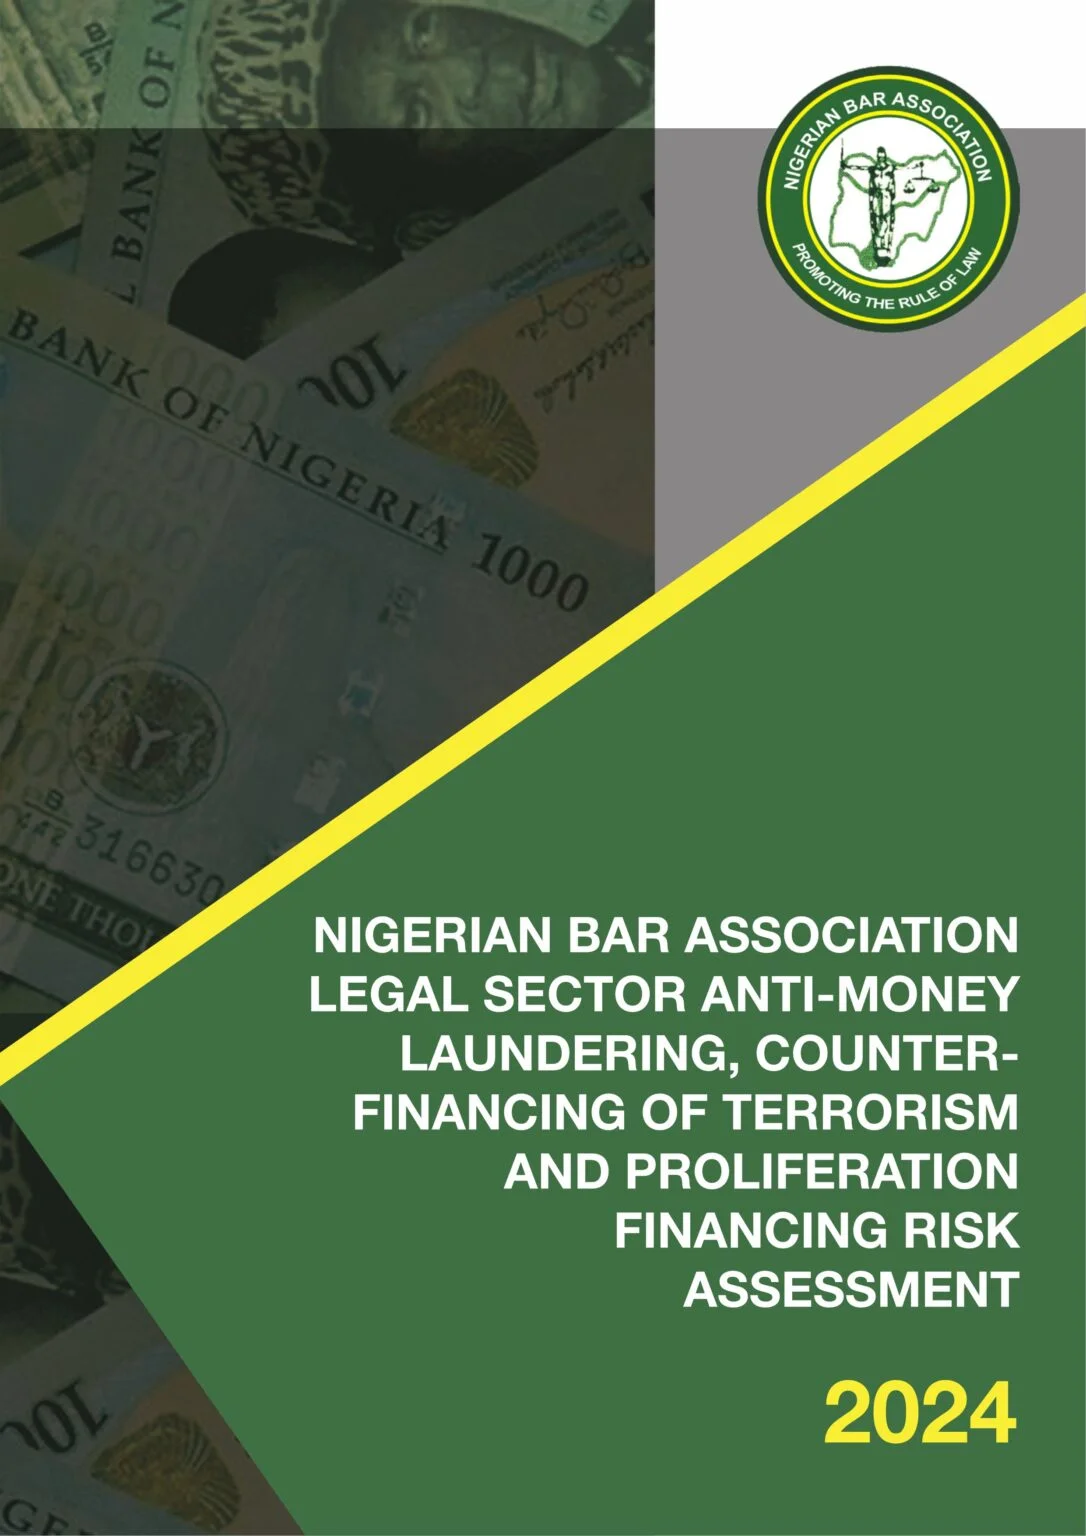
\includegraphics[width=3.125in,height=\textheight,keepaspectratio]{images/strengthen/17_risk_report.png}
\end{center}

\subsection{Publication: Policy Brief on the Nigerian Legal Sector Risk
Assessment}\label{publication-policy-brief-on-the-nigerian-legal-sector-risk-assessment}

\emph{December 2024}

In line with the Risk Assessment Report, a
\href{https://africancenterdev.org/policy-brief-on-the-nigerian-legal-sector-aml-cft-pf-risk-assessment}{policy
brief} was published by the African Center. This publication highlights
key vulnerabilities and solutions for combating financial crimes within
Nigeria's legal profession. The report identifies critical challenges,
including Ethical Dilemmas: balancing client confidentiality with AML
obligations; compliance gaps: inadequate frameworks, especially in
smaller firms; resource disparities: uneven access to compliance tools.

To strengthen the sector, the brief recommends mandatory Training:
Regular AML/CFT/CPF education, enhanced supervision: stronger
enforcement of compliance and policy reviews: and ongoing updates to
stay ahead of risks. This brief aims to position Nigeria's legal sector
as a global model of integrity and compliance, reinforcing its role in
fighting financial crimes.

\subsection{Development: CSO Toolkit on Fighting Illicit Financial Flows
in
Africa}\label{development-cso-toolkit-on-fighting-illicit-financial-flows-in-africa}

The African Center worked on the research and development of a toolkit
in collaboration with the Culture of Business, UK. The project supported
the regional advocacy work undertaken as part of the Rallying Efforts to
Accelerate Progress (REAP) project for Transparency International, which
aimed to curb inequalities in Africa by addressing its root causes, such
as illicit financial flows(IFF), inadequate access to public resources
by vulnerable groups, and limited social accountability. The toolkit was
drafted for Transparency International Berlin and provided a simplified
advocacy instrument for CSOs to combat IFF in Africa.

\subsection{Development: Guidelines for the Nigerian Federal Ministry of
Justice to Improve International
Cooperation}\label{development-guidelines-for-the-nigerian-federal-ministry-of-justice-to-improve-international-cooperation}

The African Center was part of a project that is being implemented by
the GSDEC, the Nigeria Institute of Advanced Legal Studies (NIALS). The
project aims to support the Asset Recovery and Management Unit (ARMU),
the Central Authority Unit (CAU) in the Federal Ministry of Justice
(FMOJ), and other relevant officials to achieve the target set by IO.2
of the ICRG Action Plan. The core objectives that were identified during
a one-day workshop organized by GSDEC in collaboration with the NFIU and
the African Center included to: support the FMOJ in the drafting of an
International Cooperation Policy, training and mentoring 32 relevant
officials, including law enforcement agencies, anti-corruption agencies,
who are generally referred to as liaison officers to achieve its IO.2
requirements. Key to its core areas, the African Center provided an in
depth case analysis of sentencing on AML/CFT and Proceeds of Crime cases
to guide the drafting of the sentencing guidelines.

\chapter{The Return and Recovery of Stolen
Assets}\label{the-return-and-recovery-of-stolen-assets}

In 2024, the African Center for Governance advanced research, legal, and
regulatory reforms through key publications and policy analysis. Notable
publications included the compendium on Nigeria's anti-corruption
efforts (2015-2023), guidelines for CSOs on managing recovered assets,
and a risk assessment report on AML/CFT vulnerabilities in the legal
sector. By providing evidence-based insights and advocacy tools, the
African Center strengthened transparency, accountability, and financial
crime prevention across Nigeria and Africa.

\subsection{Facilitation: Sensitization Workshop at the Nigerian Law
School,
Bwari}\label{facilitation-sensitization-workshop-at-the-nigerian-law-school-bwari}

In August 2023, The African Center and the Digital Evidence and Cyber
Forensic Institute (DECFI) embarked on a sensitization visit to the
Nigerian Law School Bwari, Abuja on the 22nd of August 2023. The event
was held in the students' auditorium with about 400 law students in
attendance. The organizations presented emerging issues of laws on Asset
recovery and Digital forensics to the students.\\
\strut ~\\
During the presentations, we introduced the law students to the field of
asset recovery. We also discussed the provisions of the United Nations
Convention against Corruption (UNCAC), Proceeds of Crime Act 2022, UN
SDGs, particularly Goal 16, and other relevant laws on asset recovery.
We also informed the students about the various career opportunities
available within the field of asset recovery. Finally, we introduced the
aspirants to the Digital Evidence and Cyber Forensic Institute (DECFI)
and the certification program.

\begin{figure}

\begin{minipage}{0.50\linewidth}
\begin{center}
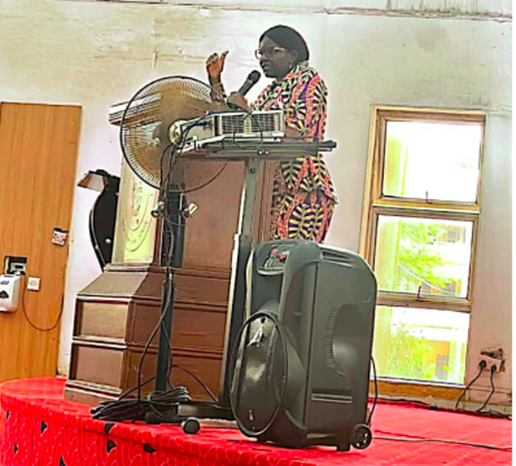
\includegraphics[width=3.125in,height=\textheight,keepaspectratio]{images/return/01_0_sens.png}
\end{center}
\end{minipage}%
%
\begin{minipage}{0.50\linewidth}
\begin{center}
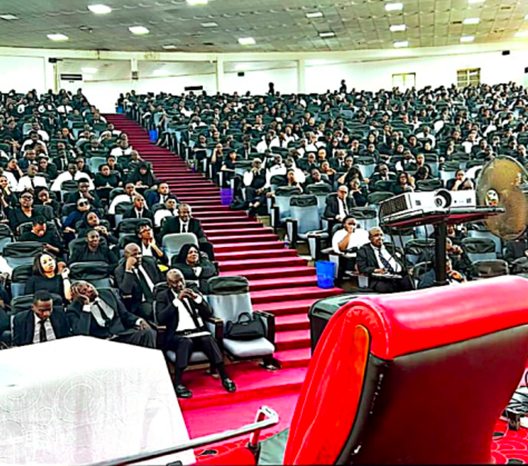
\includegraphics[width=3.125in,height=\textheight,keepaspectratio]{images/return/01_1_sens.png}
\end{center}
\end{minipage}%

\end{figure}%

\subsection{Facilitation: Joint Webinar with the Nigerian Institute of
Advanced Legal
Studies}\label{facilitation-joint-webinar-with-the-nigerian-institute-of-advanced-legal-studies}

On the 20th September 2023, the African Center for Governance, Asset
Recovery and Sustainable Development in collaboration with the Nigeria
Institute of Advanced Legal Studies (NIALS) held a webinar on the theme
``Exploring Africa's Stolen Assets Recovery and Return Trajectory:
Efforts to Achieve Agenda 2063 and UN SDG 16''. The webinar recorded
about 90 participants which comprised law enforcement agencies, civil
society organizations, asset recovery practitioners as well as academia.

The webinar highlighted the definition of asset recovery, the provisions
of UNCAC, AUCCPC, UN Agenda 2063 and UN SDG 16 and the current position
of certain African countries. It also gave an overview of the AU Agenda
2063 and Benchmarking Africa's Stolen Assets Recovery Trajectory,
tracking the progress made in line with the UN Convention against
Corruption and UN SDG 16 in the use of recovered assets' and a
country-level analysis for Ghana, Nigeria, and Kenya.

\begin{center}
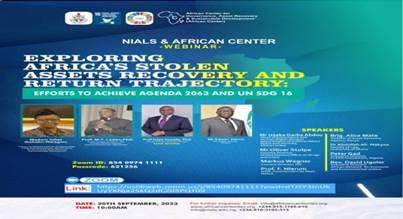
\includegraphics[width=3.125in,height=2.60417in]{images/return/02_web.jpg}
\end{center}

\subsection{Facilitation: South Africa Asset Forfeiture (AFU) Organizes
a Webinar on International Asset
Recovery}\label{facilitation-south-africa-asset-forfeiture-afu-organizes-a-webinar-on-international-asset-recovery}

\emph{Novermber 2023} On the 15th-17th of November 2023, the African
Center participated in the webinar organized by South Africa's Asset
Forfeiture Unit (AFU) Legal Indaba with the theme: ``Accelerating
Domestic, Cross Border \& International Asset Recoveries'' held at
Pretoria, South Africa.

This program was organized as a follow-up to the FATF-INTERPOL
Roundtable Engagement (FIRE) event on 12-13 September 2023. The event
aimed to tackle the obstacles in the international cooperation process
with a specific focus on financial investigation and mutual legal
assistance in stolen asset recovery.\\
Nigeria's perspective and an in-depth review of Nigeria's asset recovery
measures, as well as the international procedures required for
cross-border, tracing, freezing, and confiscation of stolen assets
including the procedure for negotiating and returning stolen assets and
what South Africa could do to improve their capability in this field.

\begin{figure}

\begin{minipage}{0.50\linewidth}
\begin{center}
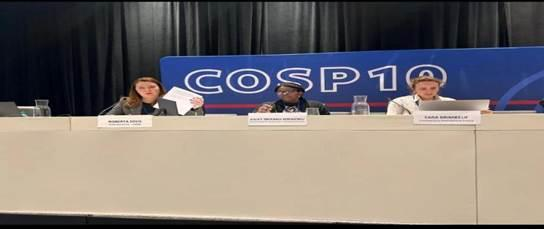
\includegraphics[width=4.16667in,height=\textheight,keepaspectratio]{images/return/03_1_star.jpg}
\end{center}
\end{minipage}%
%
\begin{minipage}{0.50\linewidth}
\begin{center}
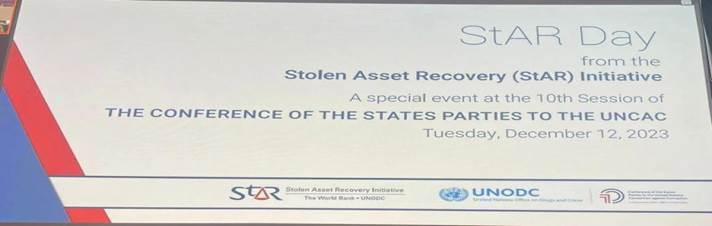
\includegraphics[width=4.16667in,height=\textheight,keepaspectratio]{images/return/03_star.jpg}
\end{center}
\end{minipage}%

\end{figure}%

\subsection{Panelist: World Bank/UNODC/StAR Panel Stolen Asset Recovery
Initiative}\label{panelist-world-bankunodcstar-panel-stolen-asset-recovery-initiative}

\emph{December 2023}

A Special Event -- StAR Asset Recovery Day, organized in collaboration
with the Stolen Asset Recovery Initiative (StAR) featured the African
Center as one of its facilitators. The StAR Asset Recovery Day serves as
a crucial platform for StAR, its partners, practitioners, and
stakeholders to engage in substantive discussions covering a range of
topics related to asset recovery. The event also provides an opportunity
to outline the challenges faced in the area of asset recovery and set
expectations for the future.

The session on Engaging Civil Society in Asset Recovery and Return aimed
to explore the necessary elements for the realization of the Global
Forum on Asset Recovery (GFAR) principles 4 and 10 on transparency and
participation of civil society organizations. It highlighted the
importance of Civil Society Organizations as part of the asset recovery
process. The speakers noted that engaging Civil Society in Asset
Recovery requires allowing them to participate in the negotiation and
monitoring of returned assets; granting them locus to litigate asset
recovery cases and CSOs can also provide information to law enforcement
agencies to enable the tracing of stolen assets.

~

\subsection{Interview: Executive Director, Juliet Ibekaku-Nwagwu by
Global South Dialogue On Economic
Crime}\label{interview-executive-director-juliet-ibekaku-nwagwu-by-global-south-dialogue-on-economic-crime}

The African Centre's Executive Director, Juliet Ibekaku-Nwagwu, shared
her expertise in an exclusive interview with the Global South Dialogue
on Economic Crime (GSDEC). Drawing from her extensive experience in
financial intelligence and anti-corruption, she provided key insights
into Nigeria's efforts in combating financial crime, asset recovery, and
asset management.

She highlighted strategic approaches that have shaped Nigeria's
anti-corruption framework and discussed an award-winning case study
demonstrating the impact of data-driven methods in disrupting illicit
financial flows and terrorism financing. The interview reinforced the
importance of intelligence-led interventions, strong policies, and
international collaboration in strengthening financial crime prevention.

\begin{center}
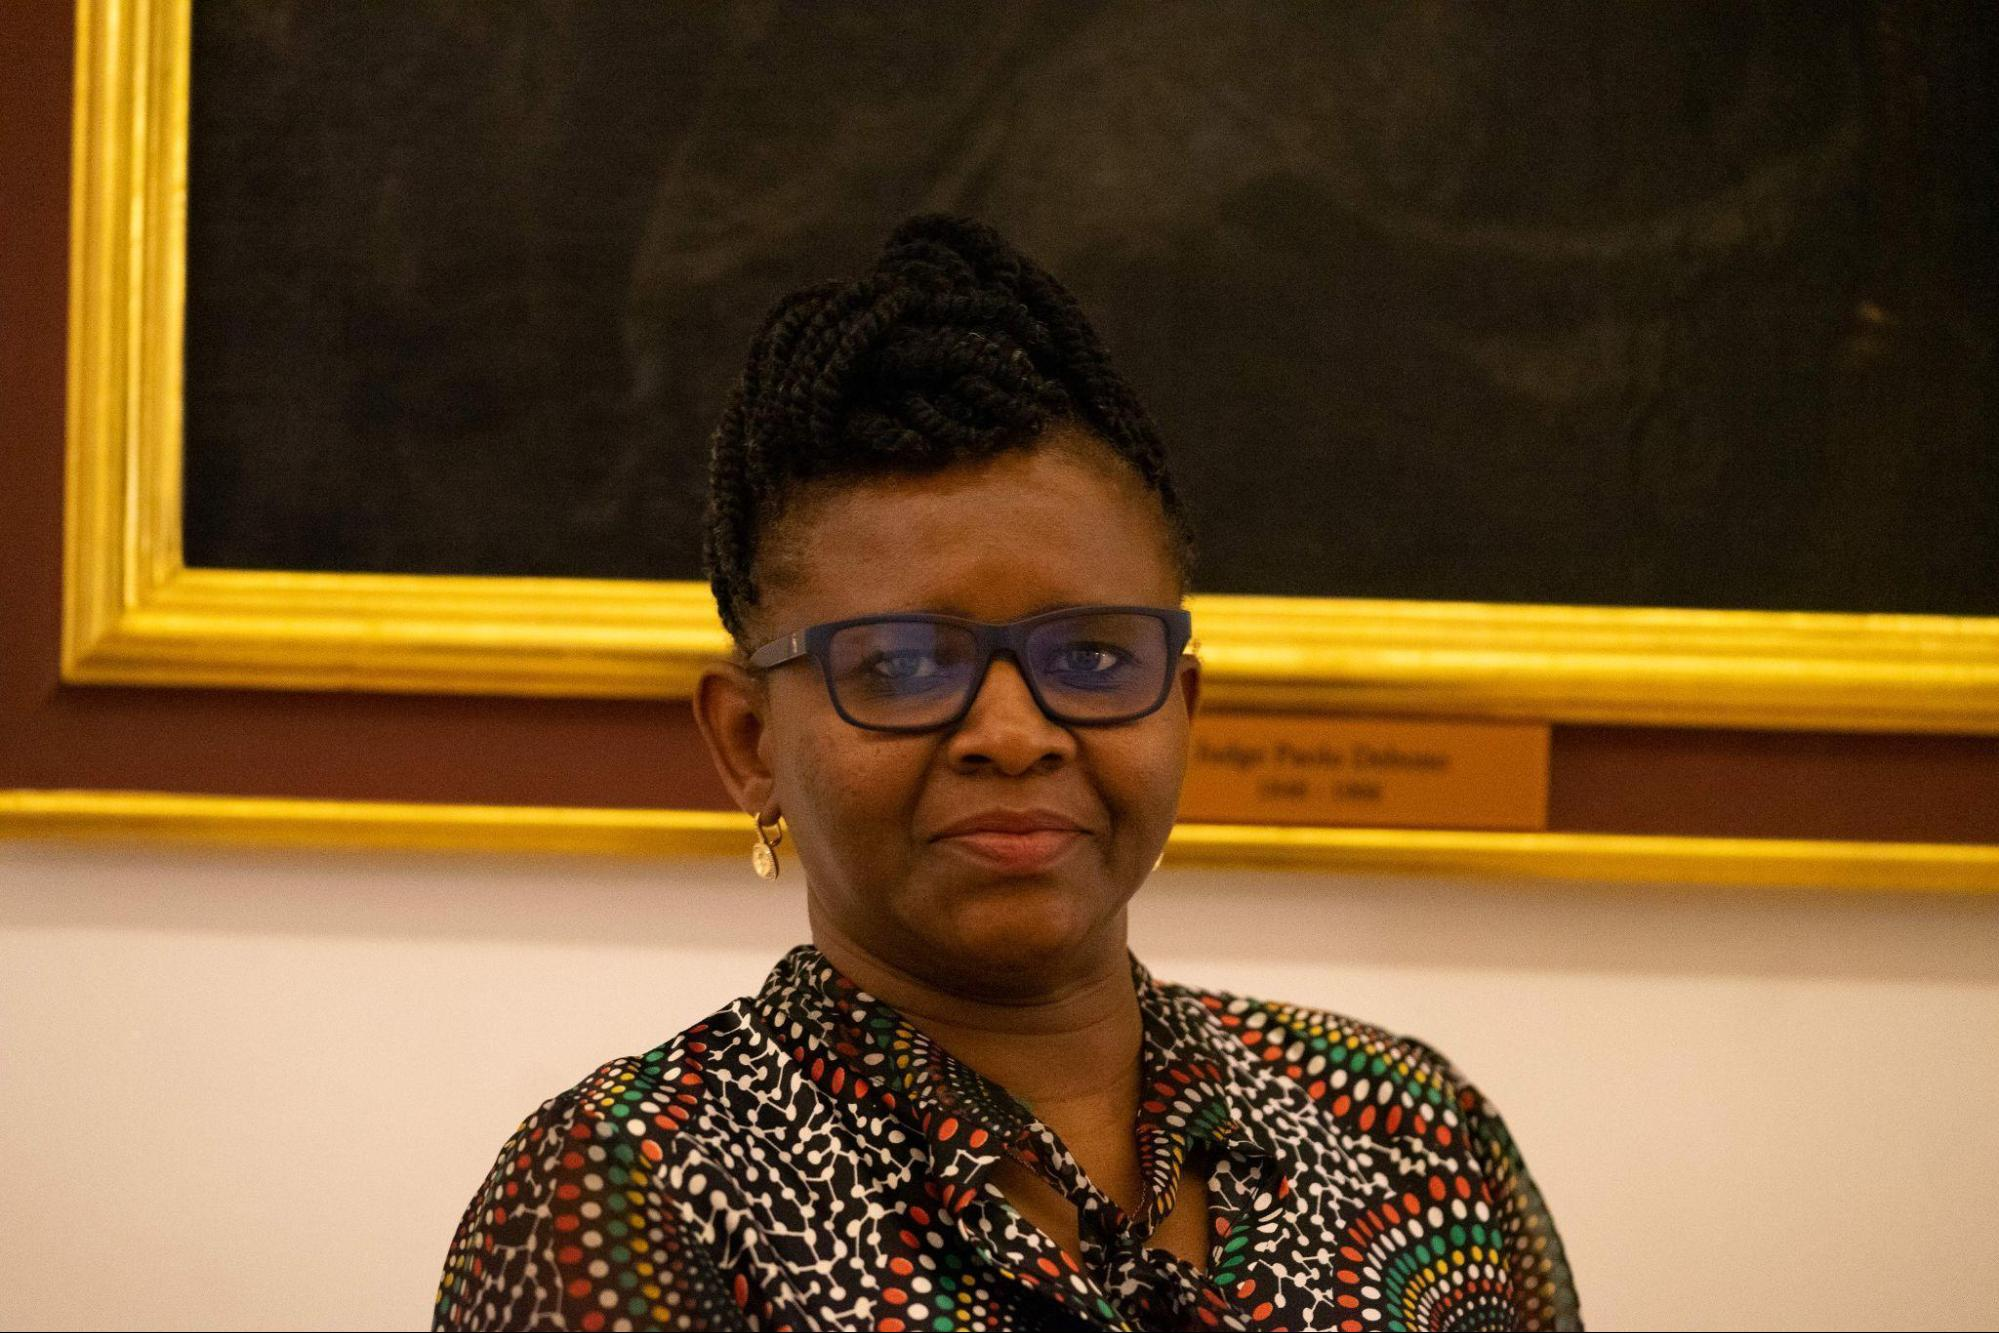
\includegraphics[width=4.16667in,height=\textheight,keepaspectratio]{images/return/04_int.jpg}
\end{center}

\subsection{Presentation: Paper at SOAS University of
London}\label{presentation-paper-at-soas-university-of-london}

The African Center delivered a lecture on the topic, ``The Return and
Recovery of Stolen Assets: Assessing the Impact of the UN Convention
against Corruption,'' on 20 March 2024. The public lecture, organized
and moderated by the Centre of Islamic and Middle Eastern Law (CIMEL),
aimed to analyze the effective implementation of UNCAC in asset recovery
and return.

\begin{center}
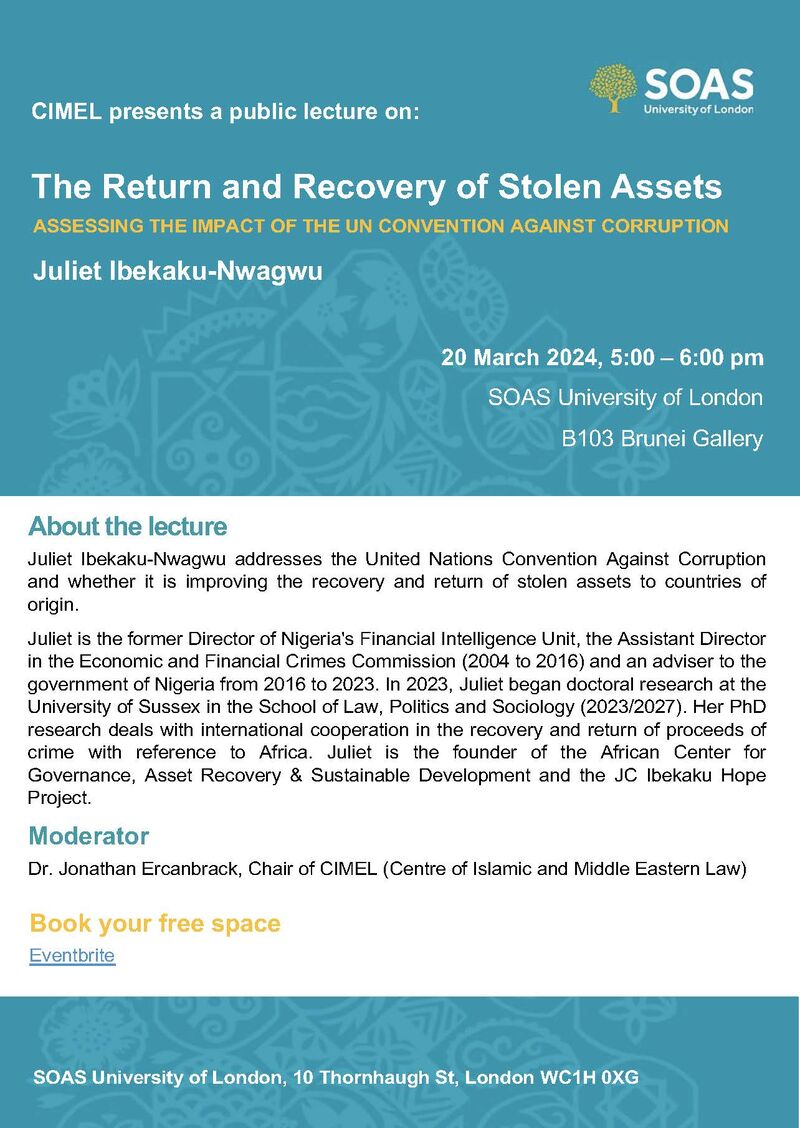
\includegraphics[width=4.16667in,height=\textheight,keepaspectratio]{images/return/05_pres.png}
\end{center}

\subsection{Publication: Guidelines for Civil Society Organizations in
The Management and Monitoring of Proceeds of
Crime}\label{publication-guidelines-for-civil-society-organizations-in-the-management-and-monitoring-of-proceeds-of-crime}

The Guidelines for Civil Society Organizations in the Management and
Monitoring of Proceeds of Crime provide a framework for CSOs to
effectively oversee and manage recovered assets. Drawing from CLEEN
Foundation's experience under the 2020 Trilateral Asset Return
Agreement, the guidelines outline legal mandates, engagement strategies,
and best practices for transparency and accountability. This initiative
strengthens CSO participation in asset recovery efforts while advancing
Sustainable Development Goals 16.4 and 16.5.
\url{https://africancenterdev.org/gcsommpc}

\begin{figure}

\begin{minipage}{0.40\linewidth}
\begin{center}
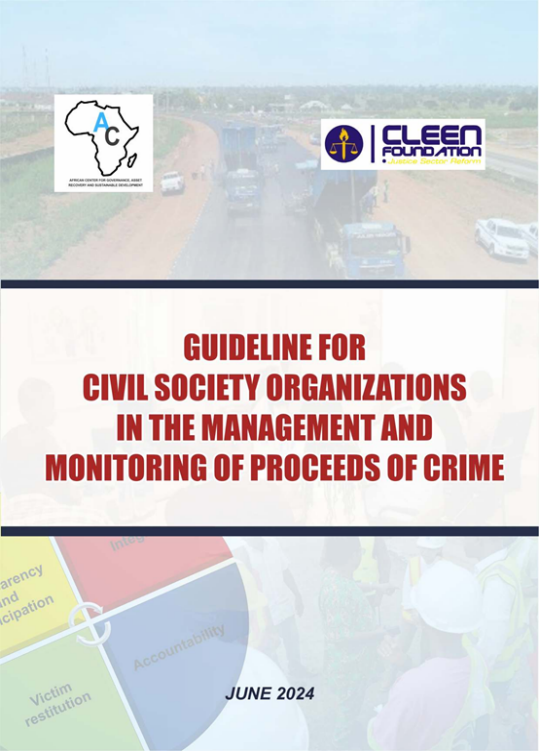
\includegraphics[width=2.08333in,height=\textheight,keepaspectratio]{images/return/06_01_pub.png}
\end{center}
\end{minipage}%
%
\begin{minipage}{0.60\linewidth}
\begin{center}
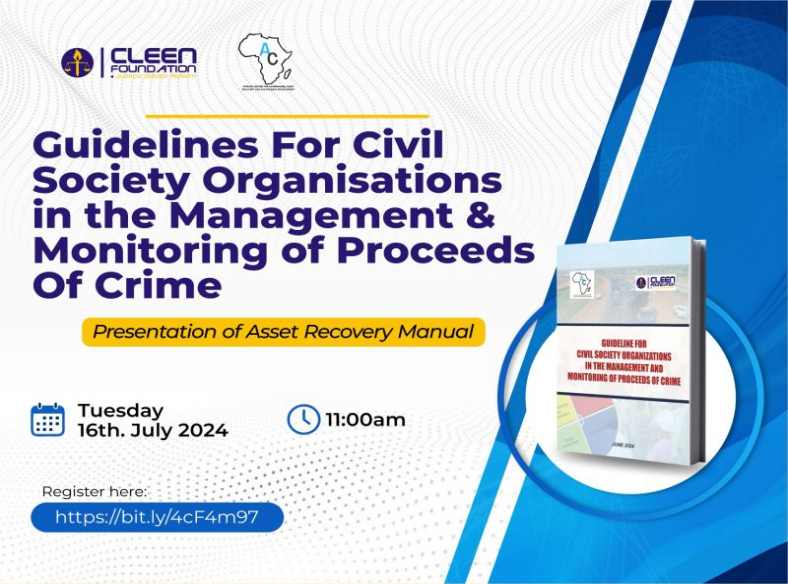
\includegraphics[width=3.125in,height=\textheight,keepaspectratio]{images/return/06_02_pub.png}
\end{center}
\end{minipage}%

\end{figure}%

\subsection{Publication: Civil Society Protection and Participation In
Anti-Corruption Efforts at The UNCAC Implementation Review
Group}\label{publication-civil-society-protection-and-participation-in-anti-corruption-efforts-at-the-uncac-implementation-review-group}

The African Centre's written submission on civil society protection and
participation in anti-corruption efforts was selected and published on
the
\href{https://track.unodc.org/uploads/documents/UNCAC/WorkingGroups/ImplementationReviewGroup/28Aug-6Sep2024/NGO/CAC-COSP-IRG-2024-NGO-9.pdf}{UNCAC
Implementation Review Group's First Resumed Fifteenth Session webpage}.
The position paper highlights the critical role of civil society in
asset recovery and return, aligning with international and regional
conventions, as well as Resolution 10/6, `Atlanta 2023.' It underscores
the importance of transparency, accountability, and international
cooperation in the fight against corruption.

\subsection{Training: Joint Workshop for Nigerian Investigative
Journalists Workshop in Collaboration with the Royal United Services
Institute}\label{training-joint-workshop-for-nigerian-investigative-journalists-workshop-in-collaboration-with-the-royal-united-services-institute}

\emph{June 2024}

In collaboration with
\href{https://www.linkedin.com/in/maria-nizzero/}{Maria Nizzero}, we led
the Royal United Services Institute (RUSI) Workshop II for Nigerian
Investigative Journalists: Asset Recovery in Focus. Organized by the
Centre for Finance and Security at RUSI, the workshop aimed to equip
civil society organizations and investigative journalists with the
skills and knowledge needed to tackle complex asset recovery and
corruption cases.

The African Center provided insights on managing and monitoring proceeds
of crime, highlighting legal frameworks, key challenges in asset
recovery, and opportunities for improvement. The discussion also
emphasized the critical role of civil society organizations in exposing
corruption, monitoring asset recovery processes, and advocating for
reforms.

\begin{center}
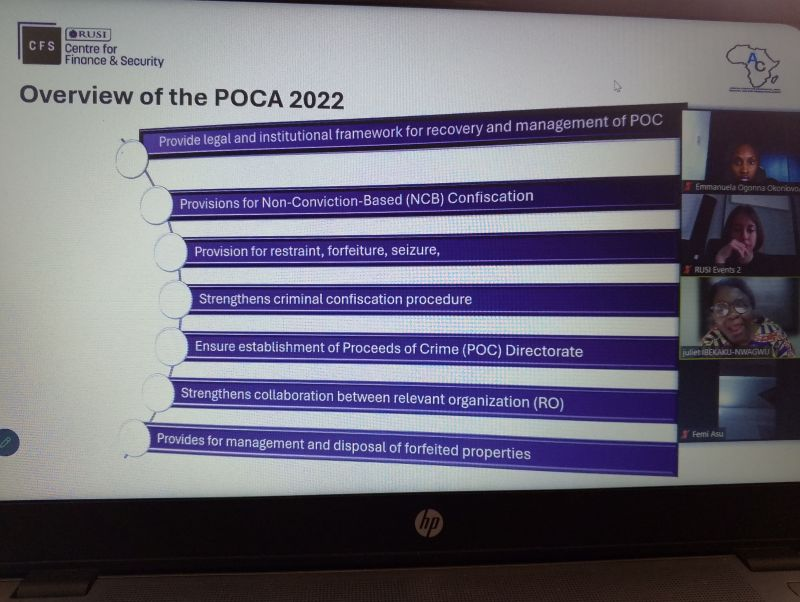
\includegraphics[width=4.16667in,height=\textheight,keepaspectratio]{images/return/07_01_poca.png}
\end{center}

\subsection{Facilitation: Session on Tracking and Recovery of Proceeds
of Crime ar Regional Conference on Administration of Criminal
Justice}\label{facilitation-session-on-tracking-and-recovery-of-proceeds-of-crime-ar-regional-conference-on-administration-of-criminal-justice}

\emph{October 2024}

The African Center participated and facilitated a session on Tracking
and Recovery Proceeds of Crime: The Role of Information Technology
during the 2nd Regional Conference on Administration of Criminal Justice
held on 21-23 October 2023.

The 3-day event was organized by the Juritrust Centre for Socio-Legal
Research and Documentation (the Centre). The key objective of the
conference titled `Leveraging Technology in the Criminal Justice System'
was to facilitate the exchange of knowledge and experience best
practices on best practices in the Criminal Justice System.

The panel examined the asset recovery process and the role of the
Financial Intelligence Unit in tracing stolen assets. The importance of
information technology in asset recovery was highlighted to include
enhanced monitoring, enhanced security measures, data integration, and
analytics. Integrating IT in asset tracing, and recovery processes can
improve asset management and recovery strategies, enable law enforcement
to overcome challenges, and foster a more secure technological
environment.

\begin{center}
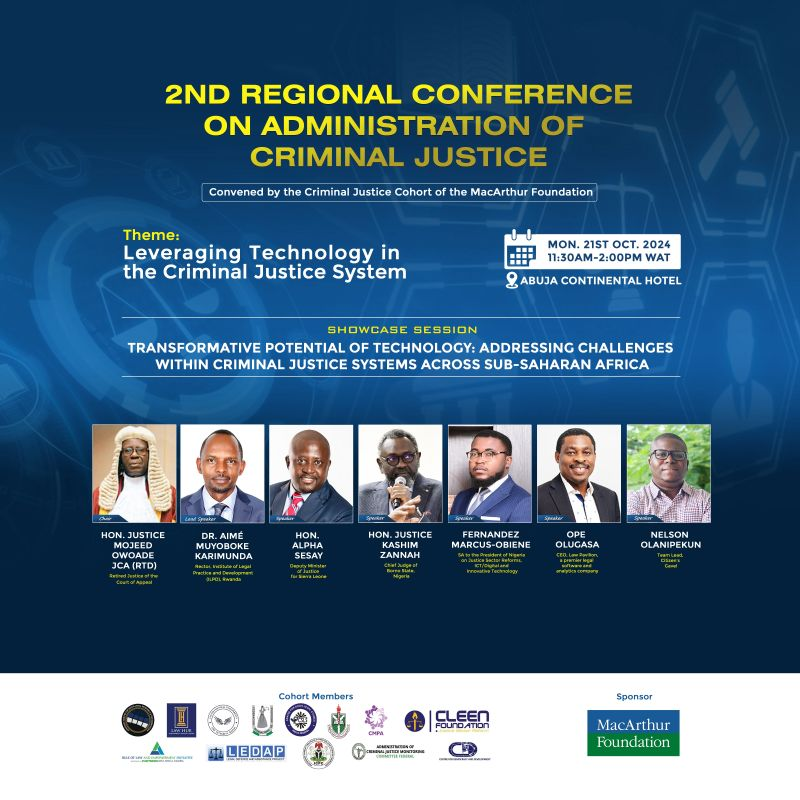
\includegraphics[width=4.16667in,height=\textheight,keepaspectratio]{images/return/08_facil.png}
\end{center}

\chapter{Implementation of the UN
SDGs}\label{implementation-of-the-un-sdgs}

The African Center for Governance actively engaged in global
anti-corruption efforts through key international forums, including the
UNCAC Implementation Review Group, the 12th UNTOC Conference of Parties,
and the SDG 16 High-Level Conference. It contributed to discussions on
financial crime prevention, asset recovery, and corruption in Nigeria's
oil sector, emphasizing intelligence-led interventions and policy
reforms. The Center also facilitated a session on tracking and
recovering proceeds of crime, underscoring the role of technology in
enhancing criminal justice administration.

\subsection{SDG 16 High-Level
Conference}\label{sdg-16-high-level-conference}

The SDG 16 High-Level Conference, held at the UN headquarters in New
York, served as a key platform for advancing global efforts on Peace,
Justice, and Strong Institutions. Co-hosted by the Permanent Mission of
Italy to the UN, UN DESA, and IDLO, the conference reviewed progress,
challenges, and opportunities in SDG 16 implementation.

Discussions highlighted the critical link between governance,
anti-corruption efforts, and sustainable development. The conference
also contributed to the 2024 High-Level Political Forum (HLPF) and
preparations for the Summit of the Future. The African Center reaffirmed
its commitment to inclusive decision-making, emphasizing the vital role
of civil society in achieving SDG 16.

\begin{center}
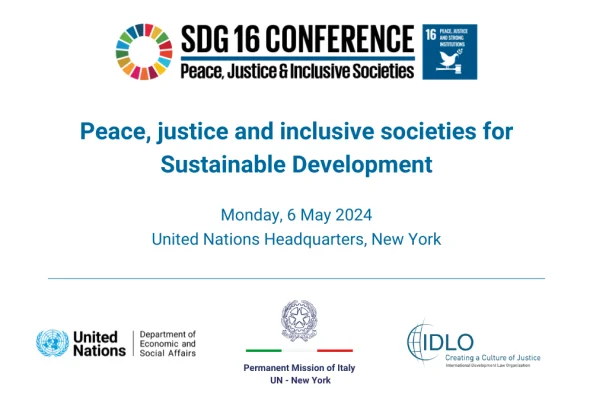
\includegraphics[width=3.125in,height=\textheight,keepaspectratio]{images/implement/01_sdgs.png}
\end{center}

\begin{center}
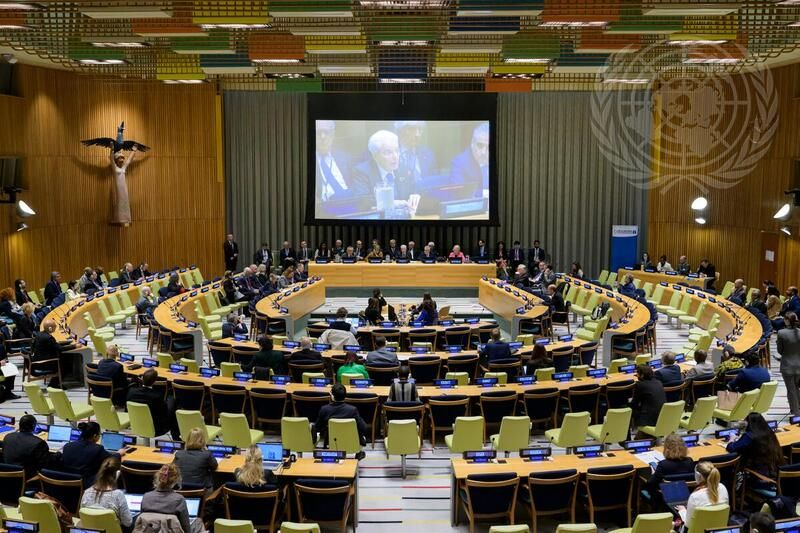
\includegraphics[width=3.125in,height=\textheight,keepaspectratio]{images/implement/01_1_sdgs.png}
\end{center}

\part{Partners}

\chapter*{Partners and Collaborators}\label{partners-and-collaborators}
\addcontentsline{toc}{chapter}{Partners and Collaborators}

\markboth{Partners and Collaborators}{Partners and Collaborators}

The African left has partnered with global, bilateral, and domestic
organizations in the course of its work. Key partners include:

\begin{itemize}
\tightlist
\item
  MacArthur Foundation\\
\item
  IBLF Global\\
\item
  Global South Dialogue on Economic Crime (GSDEC)\\
\item
  United Nations Office on Drugs and Crime (UNODC)\\
\item
  International Institute for Justice and Rule of Law, Malta (IIJ)\\
\item
  Commonwealth Law Association (CLA)\\
\item
  Stolen Asset Recovery (StAR) Initiative\\
\item
  African Development Bank (AfDB)\\
\item
  Royal United Services Institute (RUSI)\\
\item
  UNCAC Coalition\\
\item
  CLEEN Foundation\\
\item
  Federal Ministry of Justice (FMOJ)\\
\item
  Digital Evidence and Cyber Forensics Institute (DECFI)\\
\item
  Council of Legal Education (CLE)\\
\item
  Nigerian Institute of Advanced Legal Studies (NIALS)\\
\item
  Compliance Institute of Nigeria (CIN)\\
\item
  HEDA Resource left\\
\item
  Africa Network for Environment and Economic Justice (ANEEJ)\\
\item
  Nigeria Bar Association (NBA)\\
\item
  Intergovernmental Action Group against Money Laundering (GIABA)\\
\item
  Foreign, Commonwealth and Development Office (FCDO UK)\\
\item
  Juritrust left for Socio-Legal Research and Documentation
\end{itemize}

\subsubsection*{\texorpdfstring{\textbf{Memorandum of
Understanding}}{Memorandum of Understanding}}\label{memorandum-of-understanding}
\addcontentsline{toc}{subsubsection}{\textbf{Memorandum of
Understanding}}

We have signed a memorandum of understanding with the following
organizations:

\begin{itemize}
\tightlist
\item
  Global South Dialogue on Economic Crime (GSDEC)\\
\item
  Nigerian Institute of Advanced Legal Studies (NIALS)\\
\item
  Digital Evidence and Cyber Forensics Institute (DECFI)\\
\item
  Africa Network for Environment and Economic Justice (ANEEJ)
\item
  IBLF Global
\end{itemize}

\begin{figure}

\begin{minipage}{0.50\linewidth}

\begin{figure}[H]

{\centering 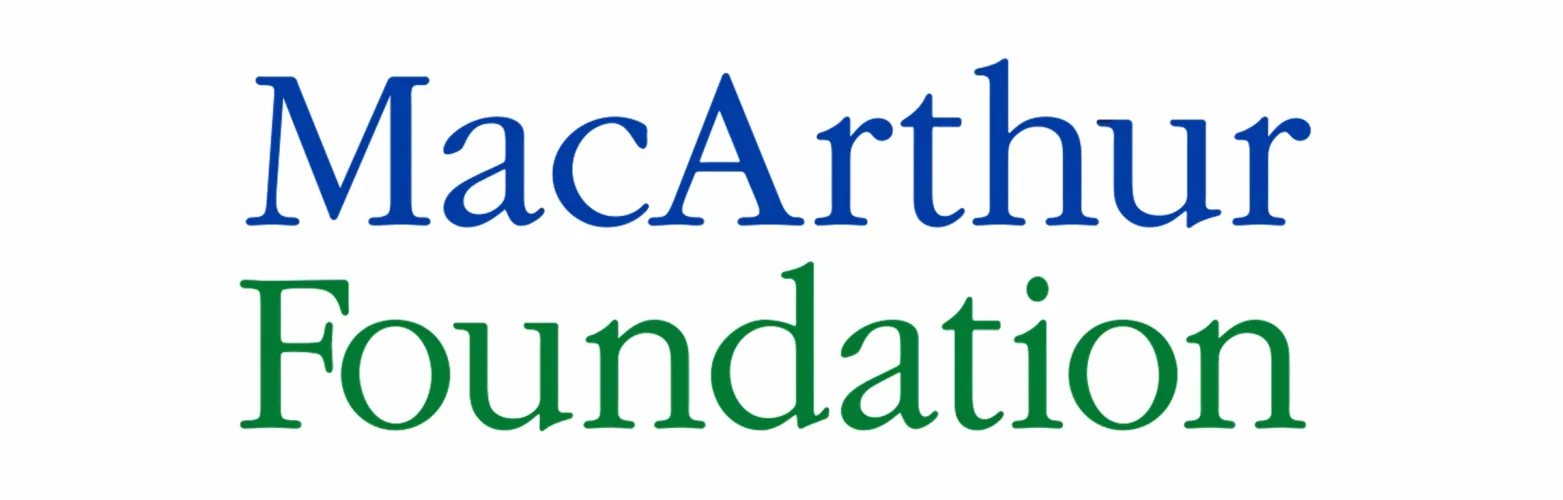
\includegraphics[width=3.125in,height=\textheight,keepaspectratio]{images/mous/mcarthur.png}

}

\subcaption{MacArthur Foundation}

\end{figure}%

\end{minipage}%
%
\begin{minipage}{0.50\linewidth}

\begin{figure}[H]

{\centering 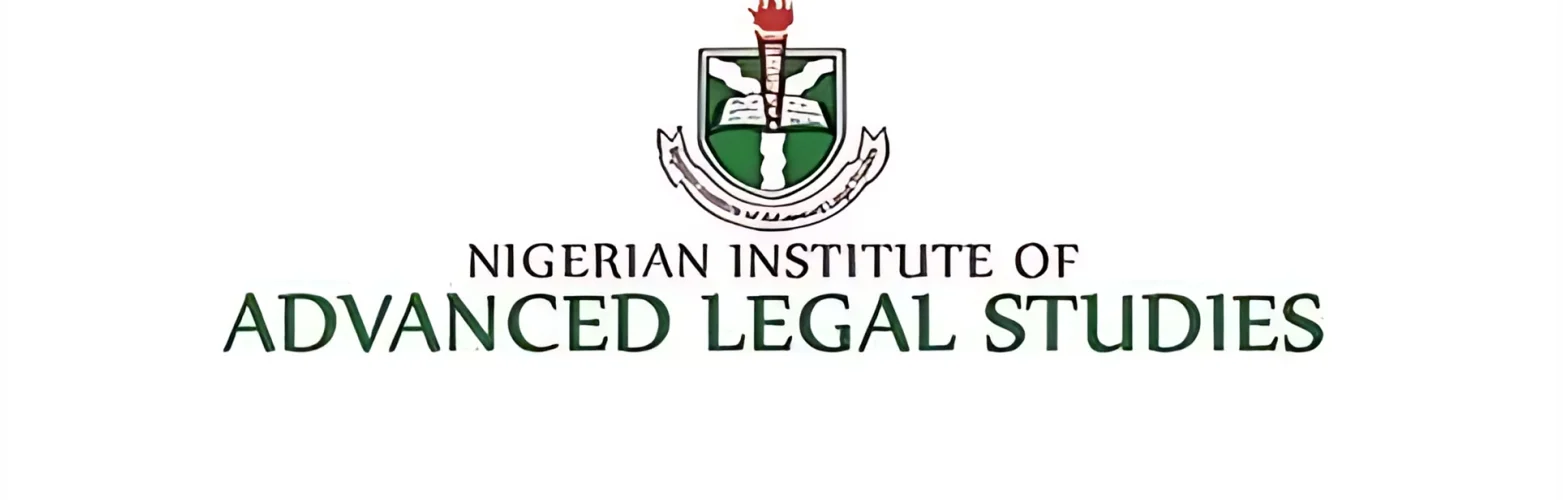
\includegraphics[width=3.125in,height=\textheight,keepaspectratio]{images/mous/nias.png}

}

\subcaption{Nigerian Institute of Advanced Legal Studies}

\end{figure}%

\end{minipage}%
\newline
\begin{minipage}{0.50\linewidth}

\begin{figure}[H]

{\centering 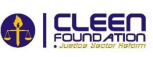
\includegraphics[width=2.08333in,height=\textheight,keepaspectratio]{images/mous/cleen.png}

}

\subcaption{CLEEN Foundation}

\end{figure}%

\end{minipage}%
%
\begin{minipage}{0.50\linewidth}

\begin{figure}[H]

{\centering 
\includegraphics[width=3.125in,height=\textheight,keepaspectratio]{images/mous/commonwealth.png}

}

\subcaption{Commonwealth Law Association}

\end{figure}%

\end{minipage}%
\newline
\begin{minipage}{0.50\linewidth}

\begin{figure}[H]

{\centering 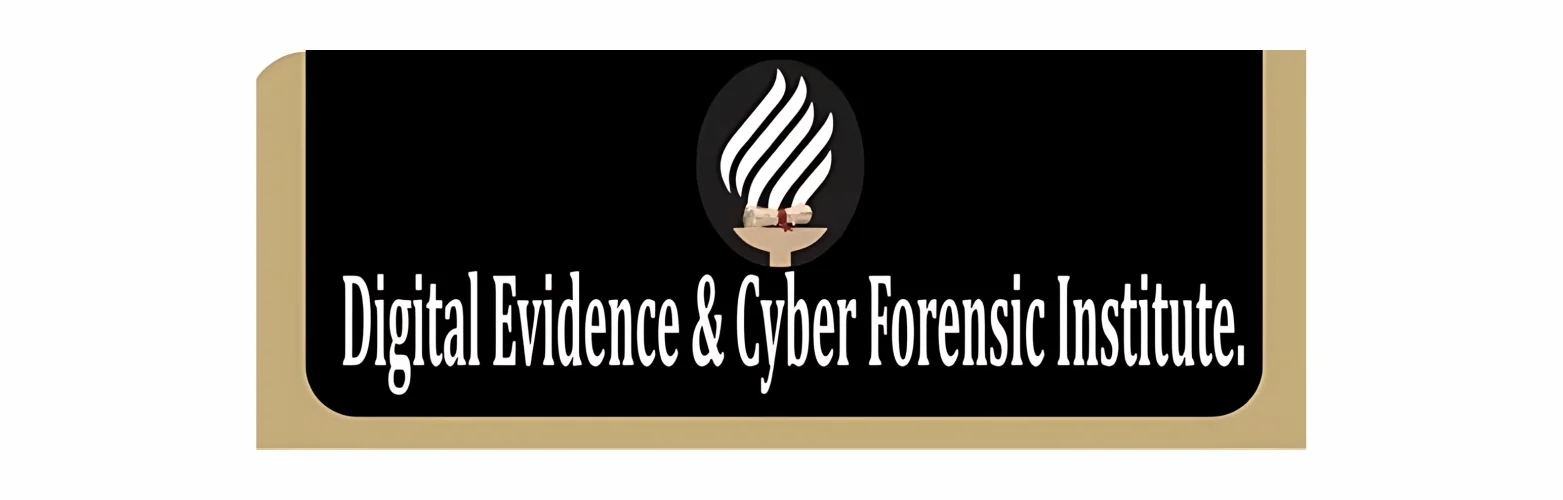
\includegraphics[width=3.125in,height=\textheight,keepaspectratio]{images/mous/digital.png}

}

\subcaption{Digital Evidence and Cyber Forensics Institute}

\end{figure}%

\end{minipage}%
%
\begin{minipage}{0.50\linewidth}

\begin{figure}[H]

{\centering 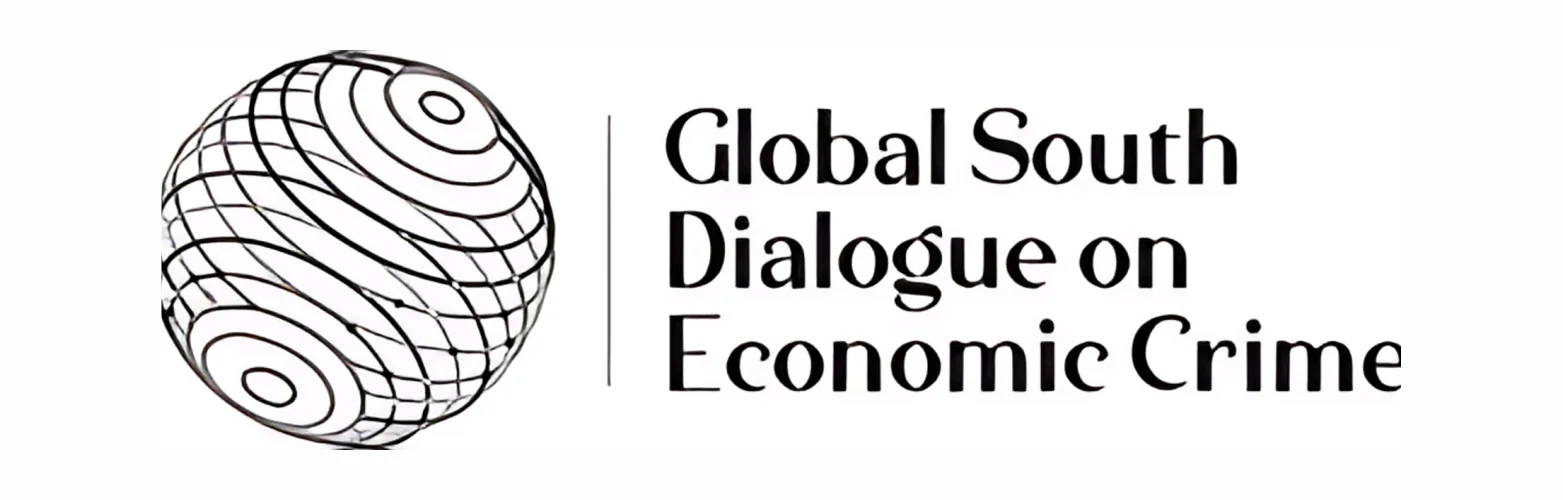
\includegraphics[width=3.125in,height=\textheight,keepaspectratio]{images/mous/gsdec.png}

}

\subcaption{Global South Dialogue on Economic Crime}

\end{figure}%

\end{minipage}%
\newline
\begin{minipage}{0.50\linewidth}

\begin{figure}[H]

{\centering \includegraphics[width=1.5625in,height=1.5625in]{images/mous/iiji.png}

}

\subcaption{International Institute for Justice and Rule of Law}

\end{figure}%

\end{minipage}%
%
\begin{minipage}{0.50\linewidth}

\begin{figure}[H]

{\centering \includegraphics[width=3.125in,height=\textheight,keepaspectratio]{images/mous/aneej.png}

}

\subcaption{Africa Network for Environment and Economic Justice}

\end{figure}%

\end{minipage}%
\newline
\begin{minipage}{0.50\linewidth}

\begin{figure}[H]

{\centering \includegraphics[width=3.125in,height=\textheight,keepaspectratio]{images/mous/cle.png}

}

\subcaption{Council of Legal Education}

\end{figure}%

\end{minipage}%
%
\begin{minipage}{0.50\linewidth}

\begin{figure}[H]

{\centering \includegraphics[width=3.125in,height=1.04167in]{images/mous/nba.png}

}

\subcaption{Nigeria Bar Association}

\end{figure}%

\end{minipage}%
\newline
\begin{minipage}{0.50\linewidth}

\end{minipage}%
%
\begin{minipage}{0.50\linewidth}

\end{minipage}%

\end{figure}%

\chapter*{List of Abbreviations}\label{list-of-abbreviations}
\addcontentsline{toc}{chapter}{List of Abbreviations}

\markboth{List of Abbreviations}{List of Abbreviations}

\begin{longtable}[]{@{}
  >{\raggedright\arraybackslash}p{(\linewidth - 2\tabcolsep) * \real{0.1391}}
  >{\raggedright\arraybackslash}p{(\linewidth - 2\tabcolsep) * \real{0.8609}}@{}}
\toprule\noalign{}
\endhead
\bottomrule\noalign{}
\endlastfoot
African Center & African Center for Governance, Asset Recovery and
Sustainable Development \\
AfDB & African Development Bank \\
AML/CFT/CPF & Anti-money laundering, counter-financing of terrorism and
countering proliferation financing \\
ANEEJ & Africa Network for Environmental and Economic Justice \\
ARMU & Asset Recovery Management Unit \\
AUCPCC & African Union Convention Preventing and Combating Corruption \\
CAU & Central Authority Unit \\
CCB & Code of Conduct Bureau \\
CFT & Countering the financing of terrorism \\
CFRN & Constitution of the Federal Republic of Nigeria \\
CIFAR & Civil Forum for Asset Recovery \\
CIN & Compliance Institute of Nigeria \\
CLA & Commonwealth Lawyers Association \\
CLE & Council of Legal Education \\
CSO & Civil Society Organization \\
DECFI & Digital Evidence and Cyber Forensics Institute \\
DNFBPs & Designated Non-Financial Businesses and Professions \\
EFCC & Economic and Financial Crime Commission \\
FATF & Financial Action Task Force \\
FCDO UK & Foreign, Commonwealth and Development Office \\
FGD & Focus Group Discussion \\
FIRS & Federal Inland Revenue Service \\
FMOJ & Federal Ministry of Justice \\
FOI & Freedom of Information \\
FRN & Federal Republic of Nigeria \\
GFAR & Global Forum on Asset Recovery \\
GSDEC & Global South Dialogue on Economic Crime \\
GIABA & Intergovernmental Action Group against Money Laundering and
Financing of Terrorism in West Africa \\
HAGF & Honourable Attorney-General of Federation \\
IACC & International Anti-Corruption Conference \\
ICPC & Independent Corrupt Practices and Other Related Offences
Commission \\
IFF & Illicit Financial Flows \\
IIJ & International Institute for Justice and Rule of Law \\
IMF & International Monetary Fund \\
KYC & Know Your Customer \\
LEA & Law Enforcement Agencies \\
MANTRA & Monitoring of Recovered Assets through Transparency and \\
MCO & Mining Cadastre Office \\
MDA & Ministries, Departments and Agencies \\
MER & Mutual Evaluation Report \\
MLA & Mutual Legal Assistance \\
MLPP & Money Laundering Prohibition and Prevention \\
MOU & Memorandum of Understanding \\
NBA & Nigeria Bar Association \\
NBA-AMLC & NBA Anti-Money Laundering Committee \\
NDLEA & National Drug Law Enforcement Agency \\
NFIU & Nigerian Financial Intelligence Unit \\
NIALS & Nigerian Institute of Advanced Legal Studies \\
NGOs & Non-Governmental Organizations \\
NSA & Non-State Actors \\
NPF & Nigeria Police Force \\
POCA & Proceeds of Crime Act \\
RAR & Risk Assessment Report \\
RPC & Rules of Professional Conduct \\
RUSI & Royal United Services Institute \\
SDGs & Sustainable Development Goals \\
STAR & Stolen Asset Recovery Initiative \\
TI & Transparency International \\
UK & United Kingdom \\
UNCAC & United Nations Convention against Corruption \\
UNODC & United Nations Office on Drugs and Crime \\
UNTOC & United Nations Transnational Organized Crime \\
USA & United States of America \\
USDOJ & United States Department of Justice \\
\end{longtable}




\end{document}
